\indent Acorde a lo solicitado, mostraremos distintos tipos de familias de casos para nuestro algoritmo, y adem\'as, daremos el tiempo estimado 
seg\'un la complejidad calculada anteriormente.\\

A continuaci\'on mostraremos un gr\'afico de tiempos comparativo entre distintas familias de casos:\\ 

\vspace*{0.3cm} \vspace*{0.3cm}
  \begin{center}
 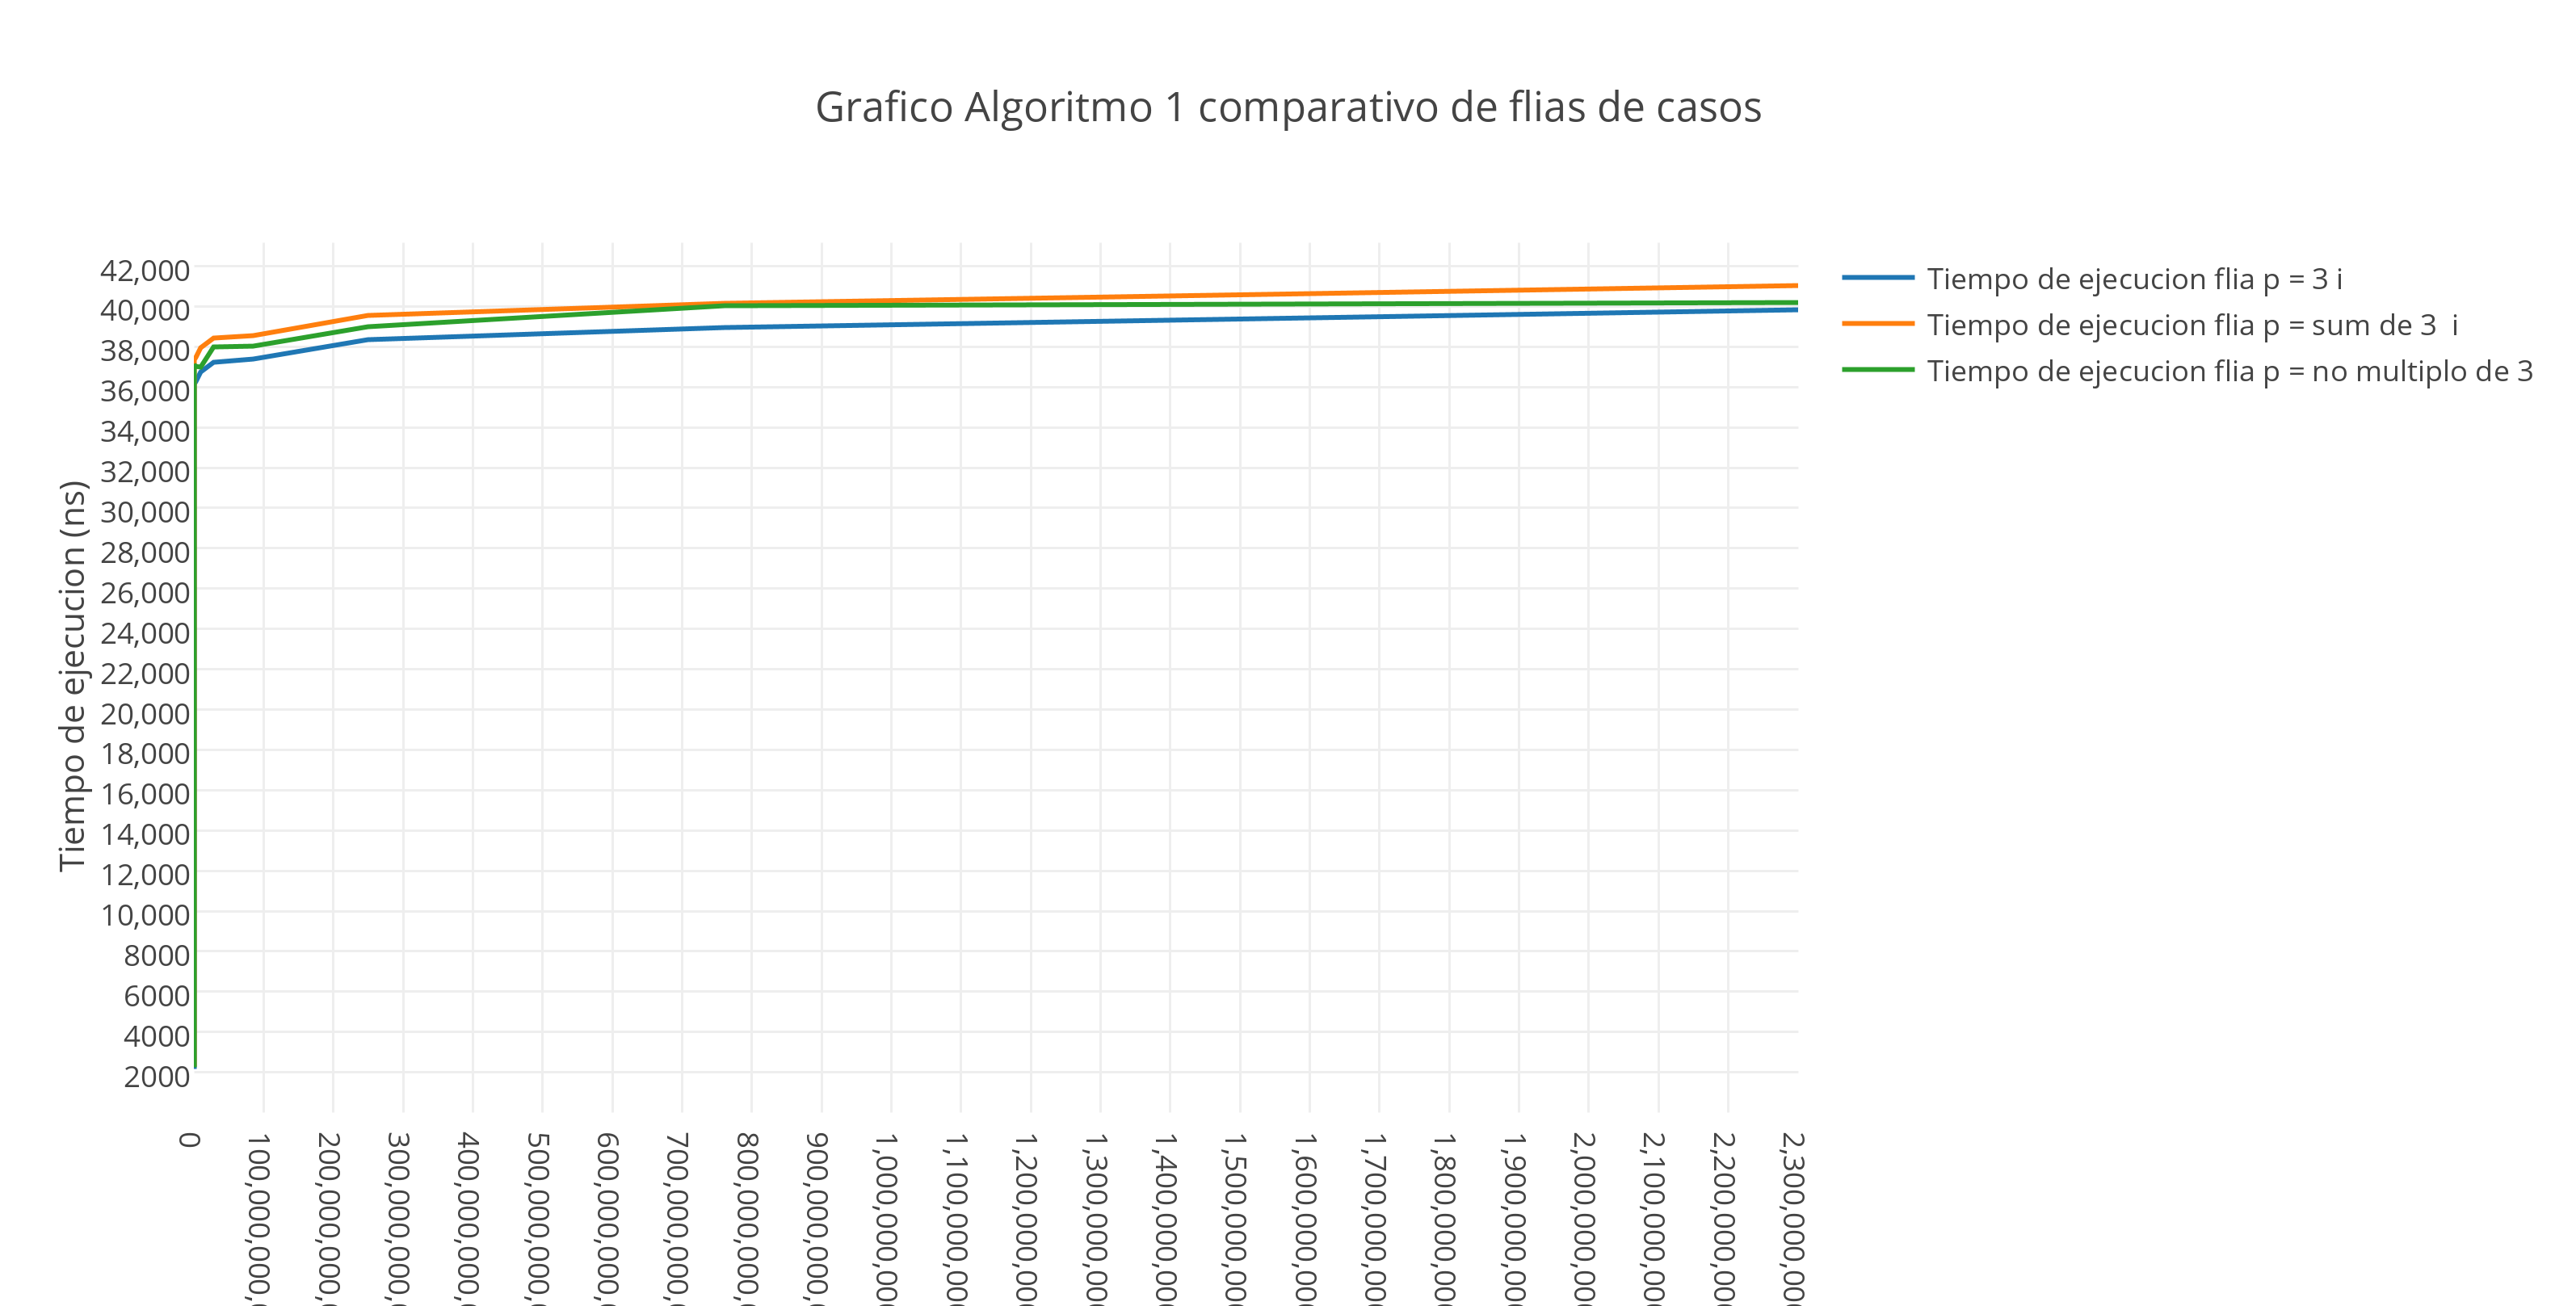
\includegraphics[scale=0.65]{./EJ2/comparativo.png}
 {$Gr$\'a$fico$ \ 2.1 - $Comparativo$}
  \end{center}
  \vspace*{0.3cm}
  
Se puede observar en el gr\'afico, tres funciones las cuales representan el tiempo de ejecuci\'on de las familias de casos:\\
\begin{itemize}
\item P es igual a una potencia de 3
\item \[
\sum_{i=1}^{n}3^{i}=P 
\]
\item P no es multiplo de 3
\end{itemize}

Como se observa en el gr\'afico la funci\'on representativa de la flia n\'umero 1, presenta una mejor performance en relaci\'on a las otras. Esto se debe a que nuestro algoritmo como va realizando sumas parciales y chequeando las potencias ve que la entrada es exactamente una \'unica potencia por lo cual toma el valor final de la suma y finaliza su ejecuci\'on, mientras que para el segundo y tercer caso, como las entradas estan dadas por varias combinaciones de potencias indudablemente se necesitar\'a para obtener dicha combinaci\'on recorrer todo el arreglo de sumas parciales m\'as de una vez.

Luego de chequear dichas instancias, pudimos llegar a la conclusi\'on que la familia de casos que presenta una mejor performance es en la cual se recibe $P$ con un valor exactamente igual a $3^i$ con 0 $\leq$ i $\leq$ n \\

Para llegar a dicha conclusi\'on trabajamos con 30 instancias ya que $3^{30}$ es el ultimo valor dentro del valor que puede tomar $P$.\\

Para una mayor observaci\'on desarrollamos el siguiente gr\'afico con las instancias:\\

\vspace*{0.3cm} \vspace*{0.3cm}
  \begin{center}
 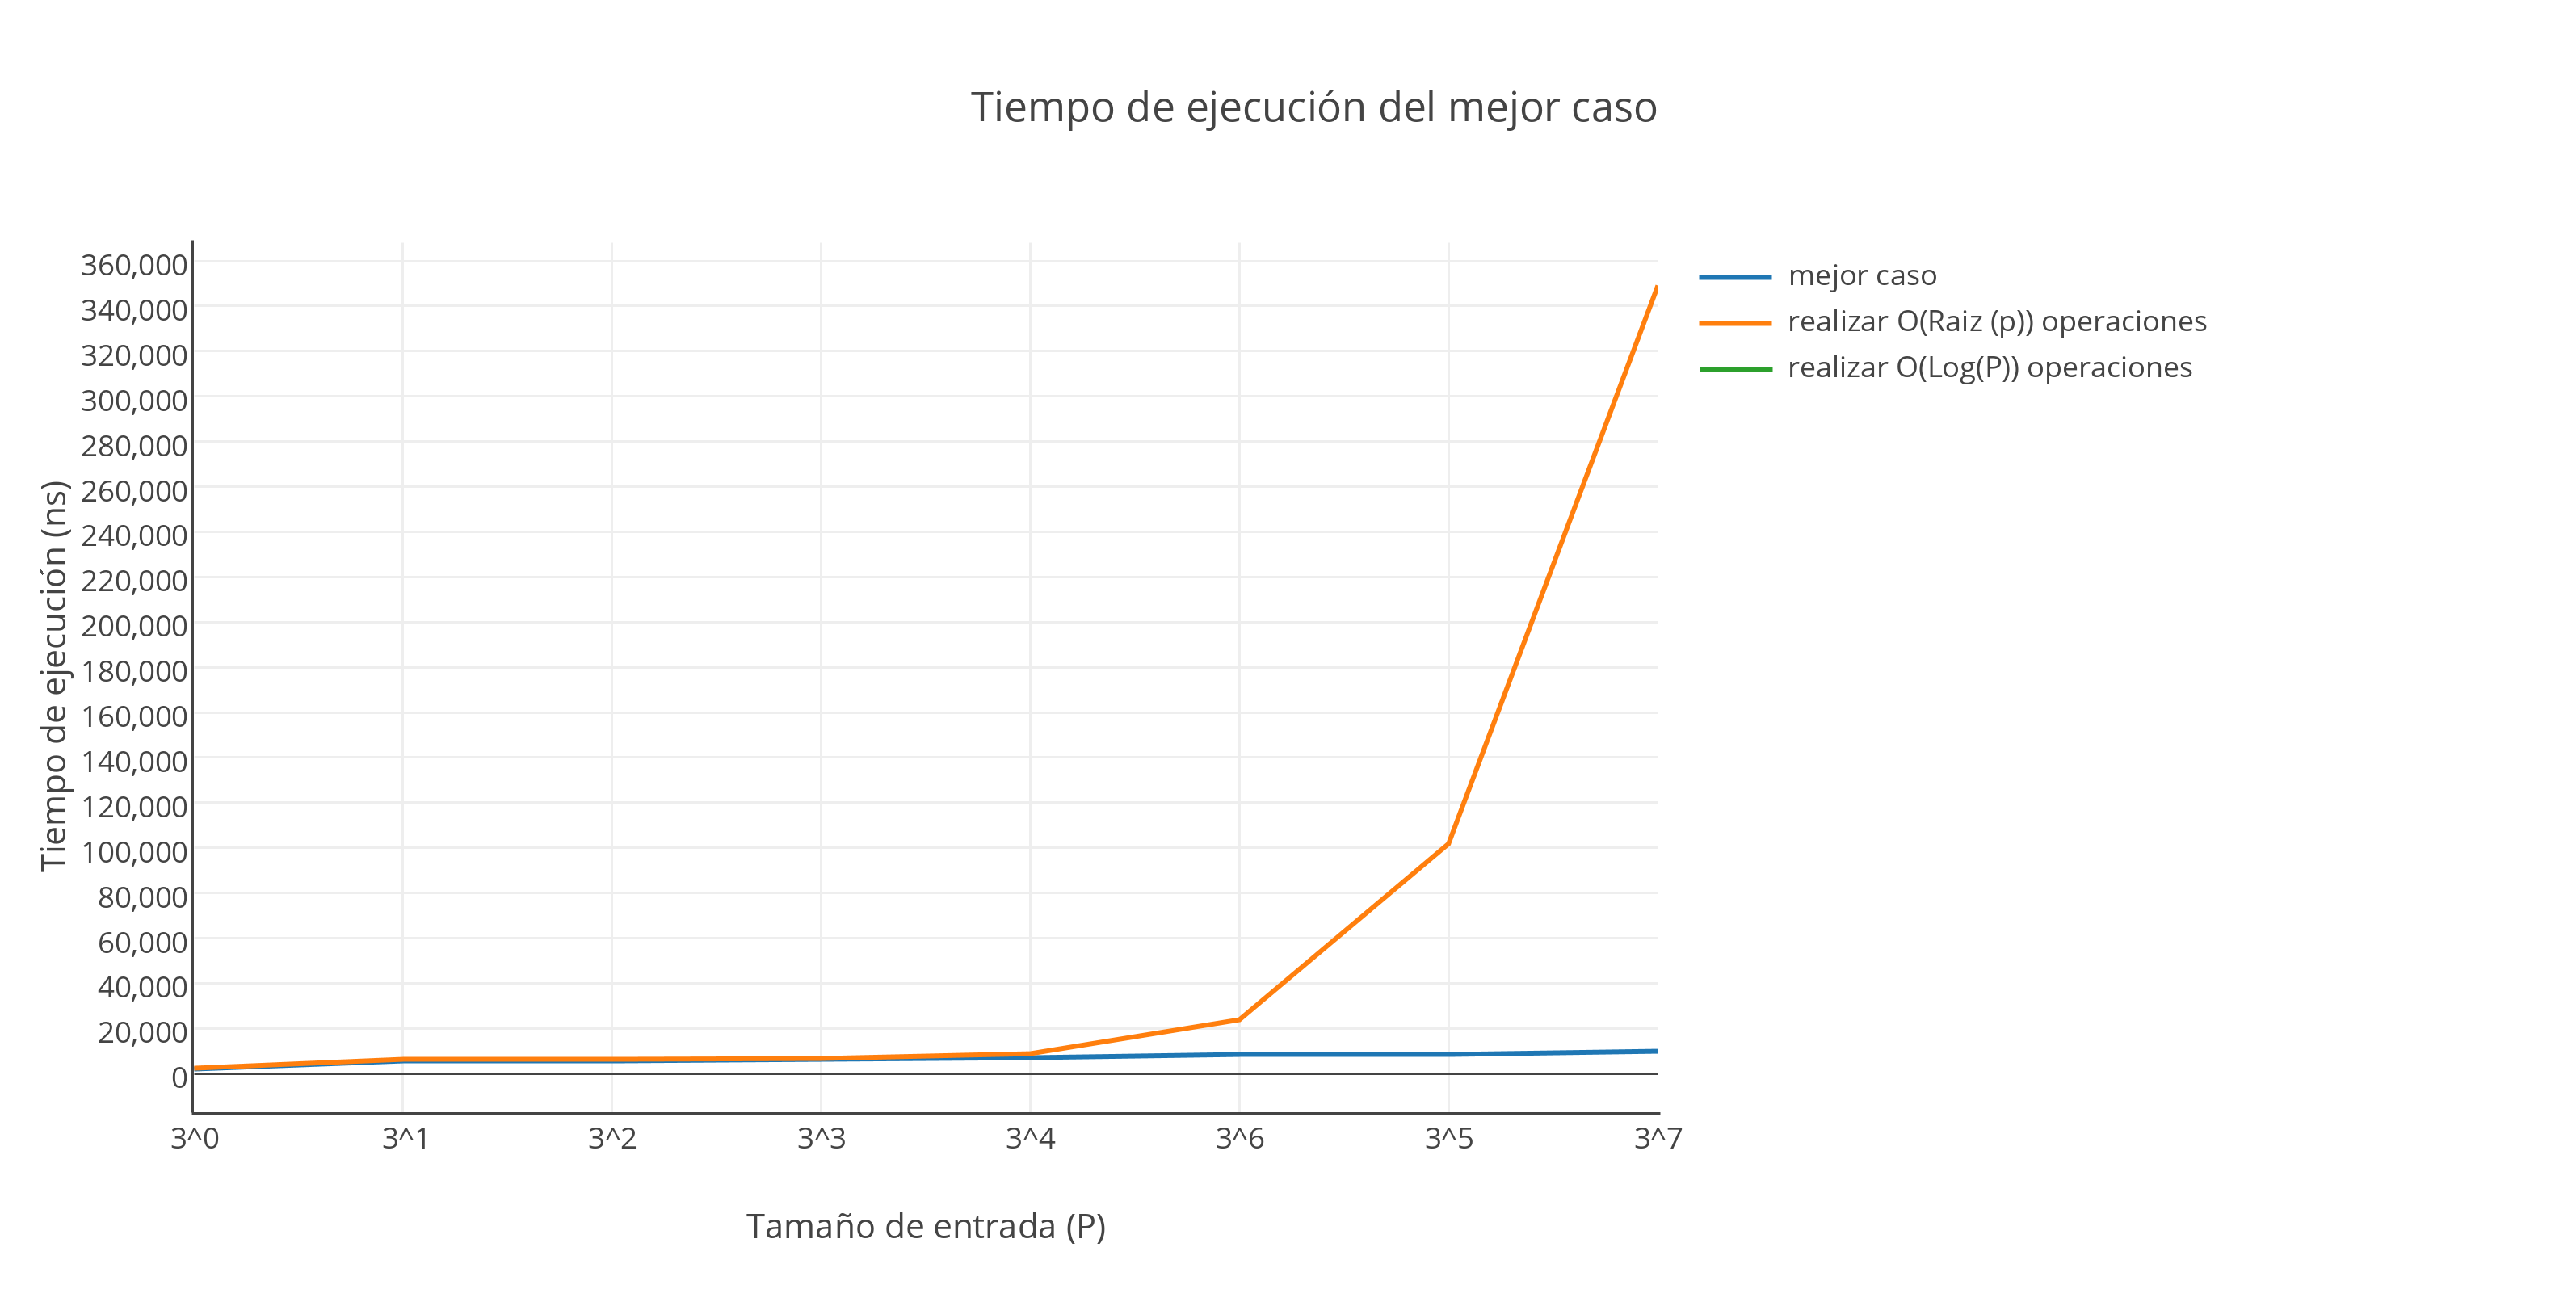
\includegraphics[scale=0.65]{./EJ2/mejorcaso.png}
 {$Gr$\'a$fico$ \ 2.1 - $Mejor Caso$}
  \end{center}
  \vspace*{0.3cm}
  
Como es posible observar en el gr\'afico, la funci\'on resultante de la cota teorica crece mucho m\'as r\'apido que la de nuestro algoritmo la cual se tiende a ser constante, es por esto que a la hora de realizar el gr\'afico de mediciones se tomaron los primeros valores debido a que, cuando la funci\'on de $\sqrt{P}$ toma valores muy grandes la misma es imposible de graficar contra nuestro algoritmo.

Adem\'as, como se puede apreciar debido a lo comentado no es posible apreciar las diferencias entre nuestro algoritmo y la cota O(Log(P)) es por esto que mostraremos un gr\'afico entre ambos:\\

\vspace*{0.3cm} \vspace*{0.3cm}
  \begin{center}
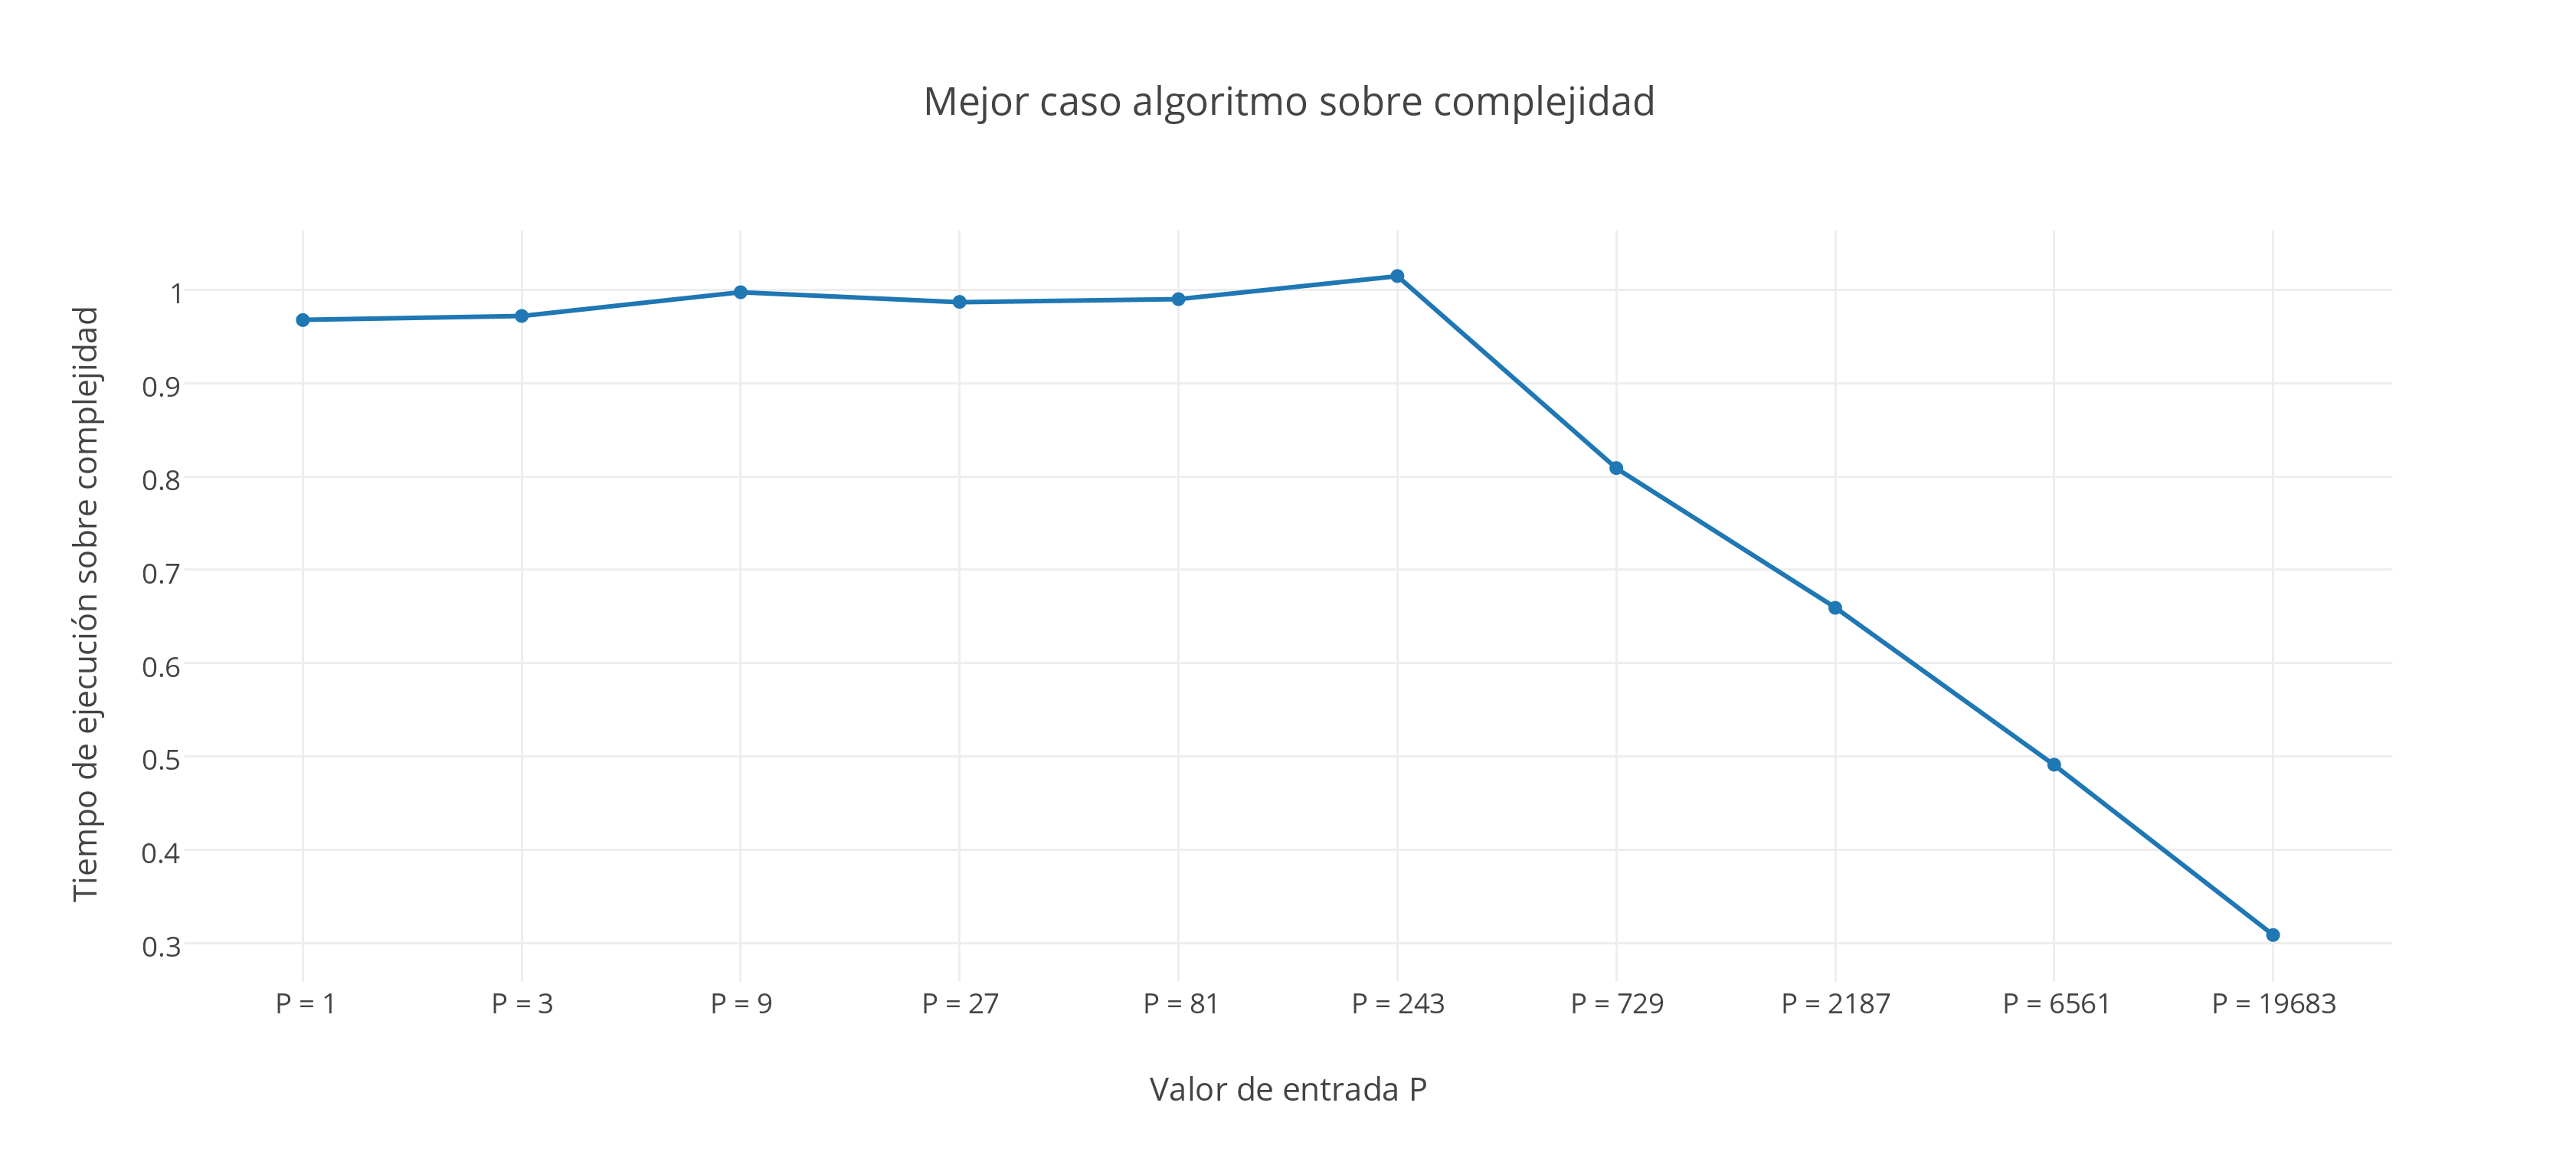
\includegraphics[scale=0.65]{./EJ2/mejorcaso2.png}
{$Gr$\'a$fico$ \ 2.3 - $Mejor Caso$}
  \end{center}
  \vspace*{0.3cm}


Luego, dividiendo por la complejidad teorica de nuestro algoritmo llegamos a:\\

\vspace*{0.3cm} \vspace*{0.3cm}
  \begin{center}
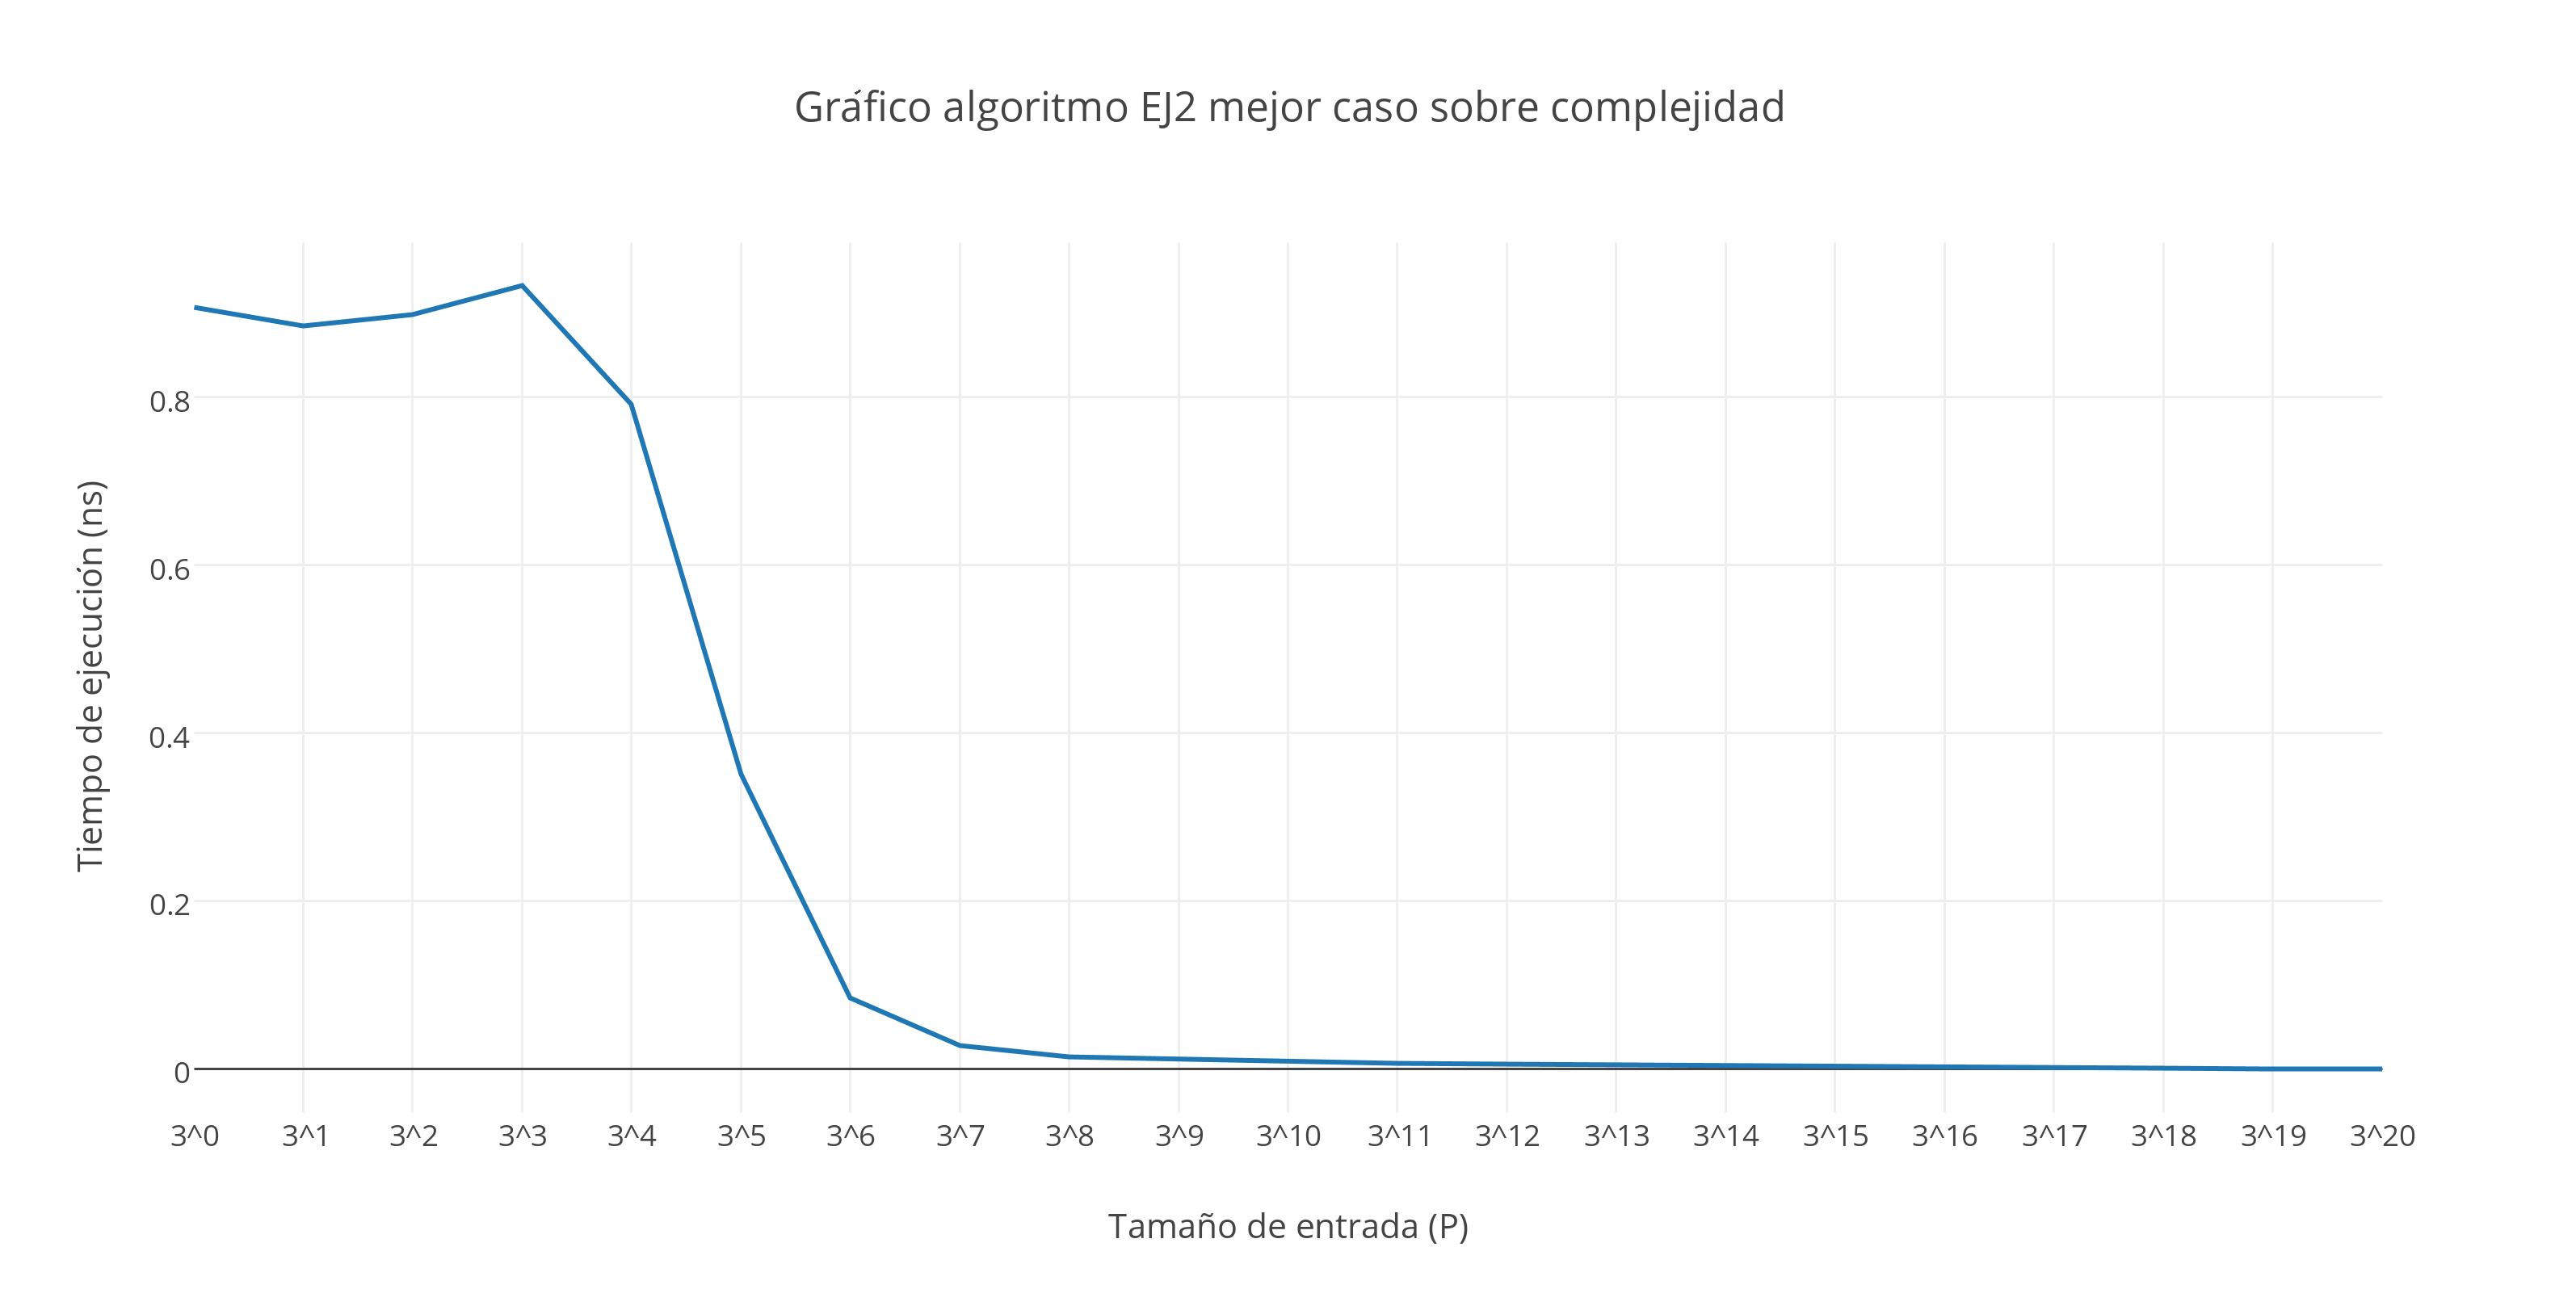
\includegraphics[scale=0.65]{./EJ2/mejorcaso1.png}
{$Gr$\'a$fico$ \ 2.4 - $Mejor Caso / Complejidad$ $O(\sqrt{P})$}
  \end{center}
  \vspace*{0.3cm}

\vspace*{0.3cm} \vspace*{0.3cm}
  \begin{center}
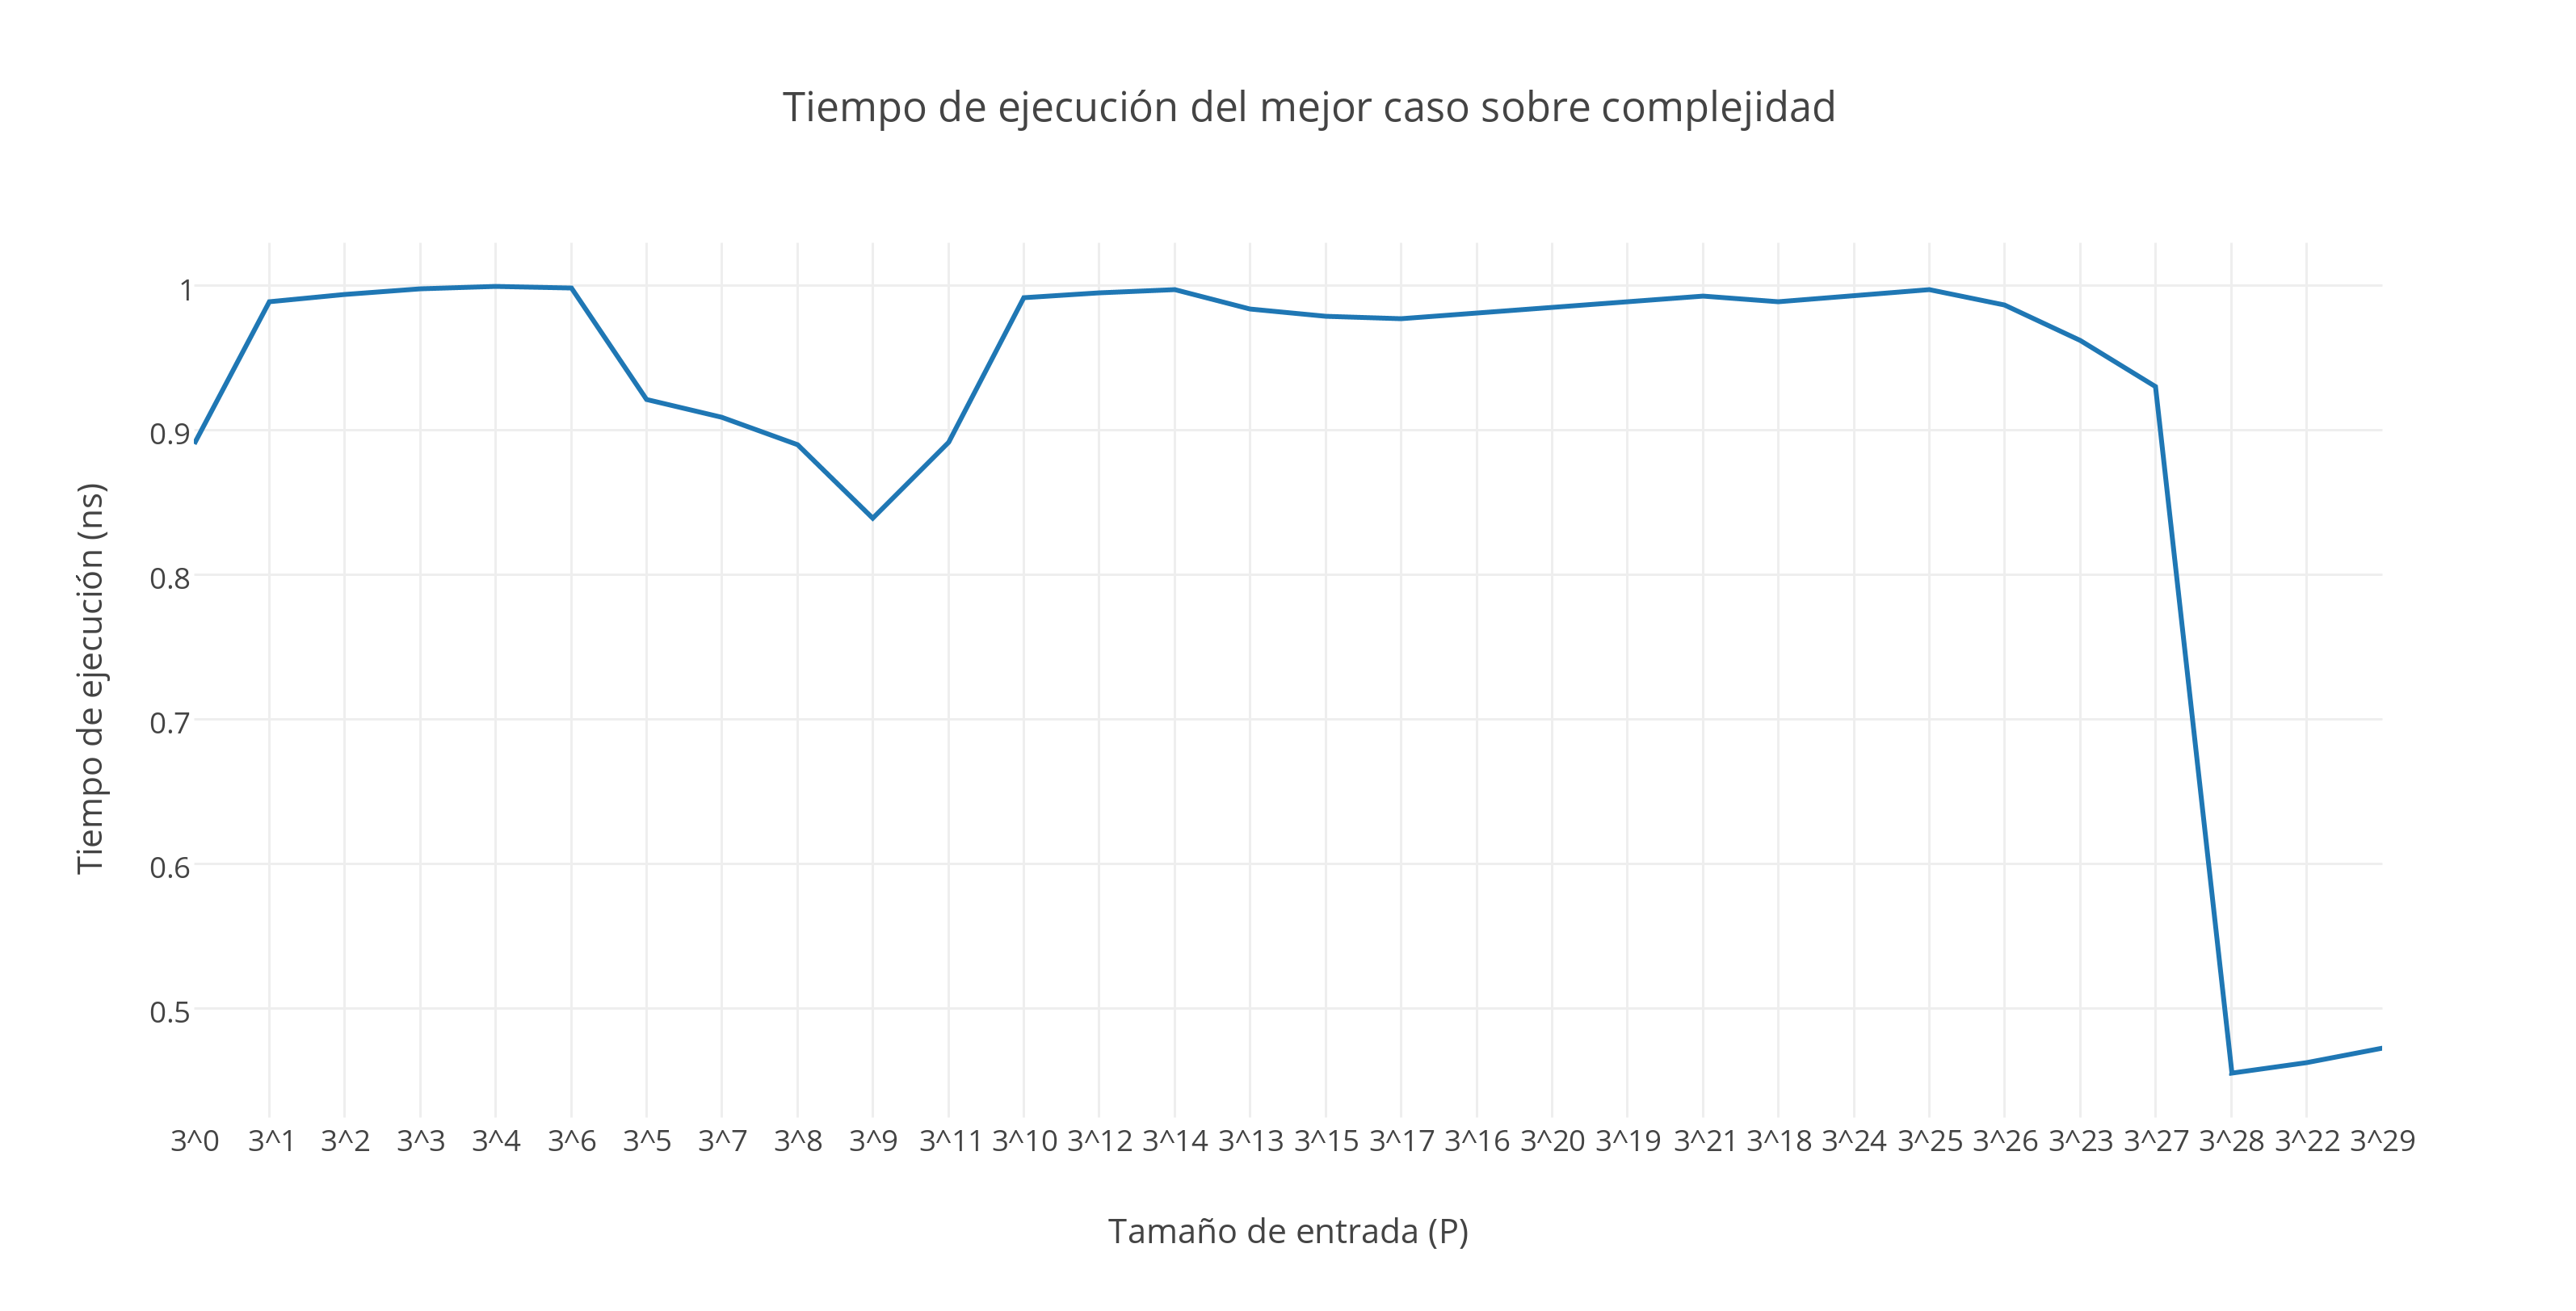
\includegraphics[scale=0.65]{./EJ2/mejorcaso3.png}
{$Gr$\'a$fico$ \ 2.4 - $Mejor Caso / Complejidad$ $O(log(P))$}
  \end{center}
  \vspace*{0.3cm}

Para realizar esta experimentaci\'on nos parecio prudente, realizar un promedio con el mismo input de aproximadamente 20 corridas
tanto para la complejidad como para nuestro algoritmo y una vez calculado dicho promedio de ambas cosas realizamos la divisi\'on para
obtener resultados m\'as relevantes.\\ 

Se puede observar en el gr\'afico 2.4, como luego de realizar la divisi\'on por la complejidad cuando el n aumenta el valor tiende a 0, tomando un valor m\'aximo en 0.93. Y, en el gr\'afico 2.4 se ve como la funci\'on resultante tiene picos en los cuales llega a un m\'aximo igual a 1 y cuando el valor de entrada aumenta la funci\'on tiende a 0.5. Por lo tanto, podemos concluir que para el mejor caso nuestro algoritmo se encuentra considerablemente por debajo de la cota teorica $O(\sqrt{P})$ y asintotizado por la cota $O(log(P))$\\

Luego, verificando el peor caso, llegamos a la conclusi\'on que la familia de casos con las que resulta menos beneficioso trabajar ser\'a cuando el valor de entrada $P$ sea de la forma \[
\sum_{i=1}^{n}3^{i}=P 
\].
\\

Realizando experimentos con un total de 20 instancias donde \[
\sum_{i=1}^{20}3^{i}=5230176601 
\], desarrollamos dos gr\'aficos los cuales mostraremos a continuaci\'on: \\

\vspace*{0.3cm} \vspace*{0.3cm}
  \begin{center}
 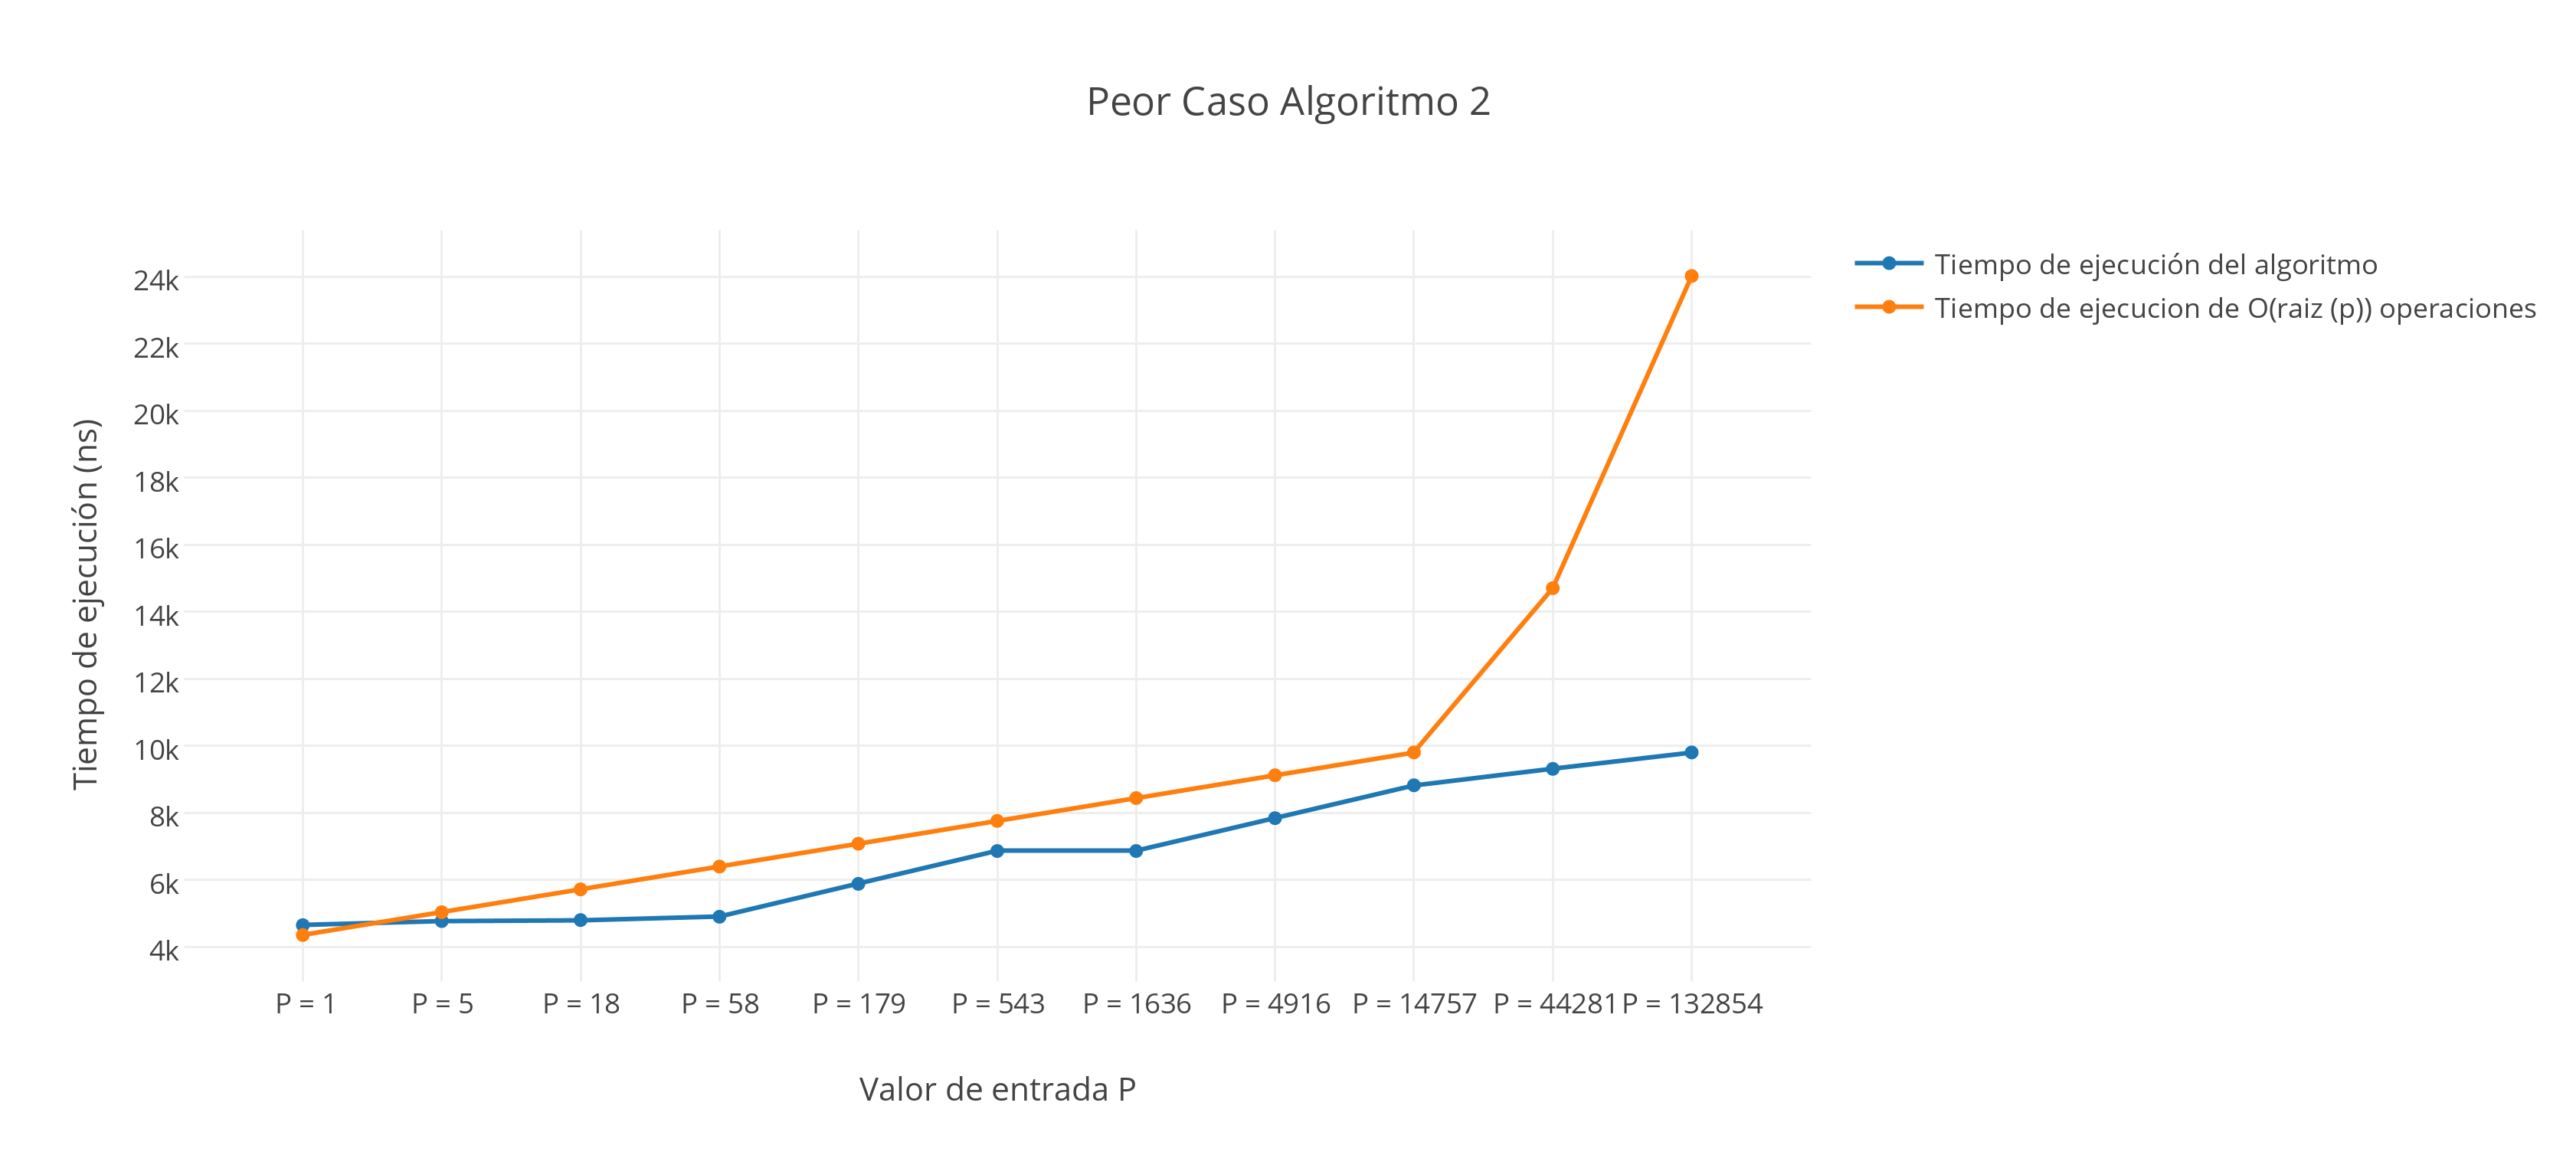
\includegraphics[scale=0.65]{./EJ2/peorcaso.png}
 {$Gr$\'a$fico$ \ 2.5 - $Peor Caso$}
  \end{center}
  \vspace*{0.3cm}

Se puede observar como la funci\'on representante de nuestro algoritmo y de $O(Log(P))$ es mucho mejor que $O(\sqrt{P})$ es por esto que realizamos un gr\'afico entre nuestro algoritmo y $O(Log(P))$

\vspace*{0.3cm} \vspace*{0.3cm}
  \begin{center}
 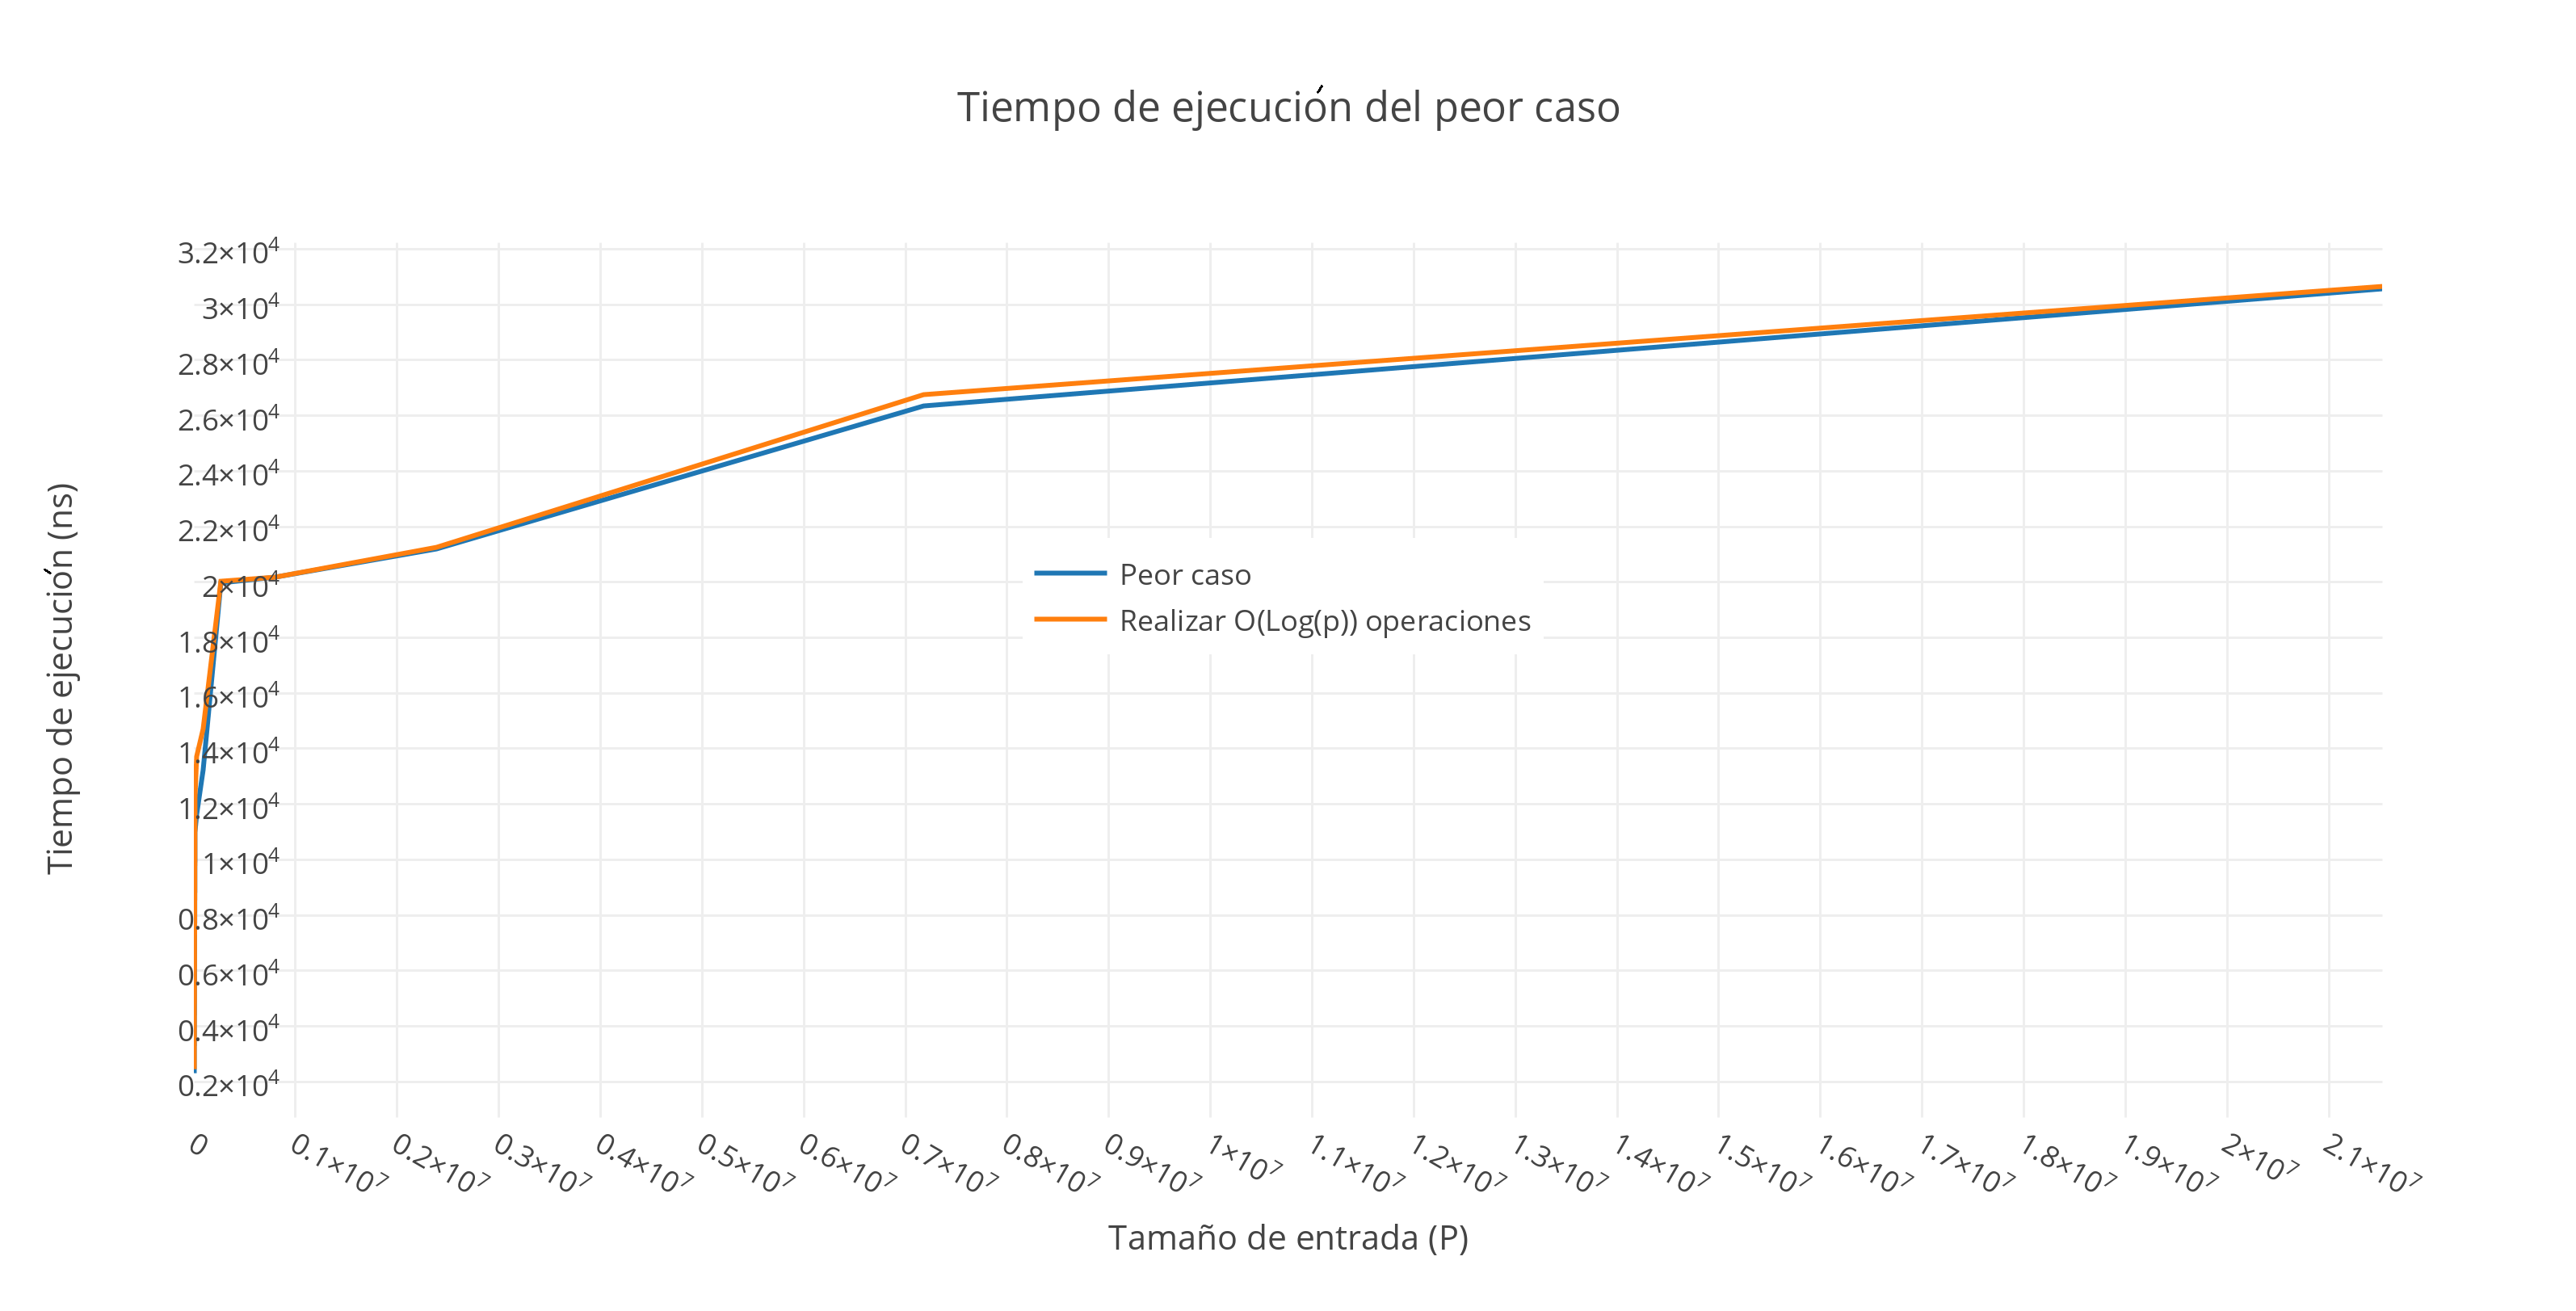
\includegraphics[scale=0.65]{./EJ2/peorcaso1.png}
 {$Gr$\'a$fico$ \ 2.6 - $Peor Caso$}
  \end{center}
  \vspace*{0.3cm}

Dividiendo por la complejidad propuesta llegamos a:\\

\vspace*{0.3cm} \vspace*{0.3cm}
  \begin{center}
 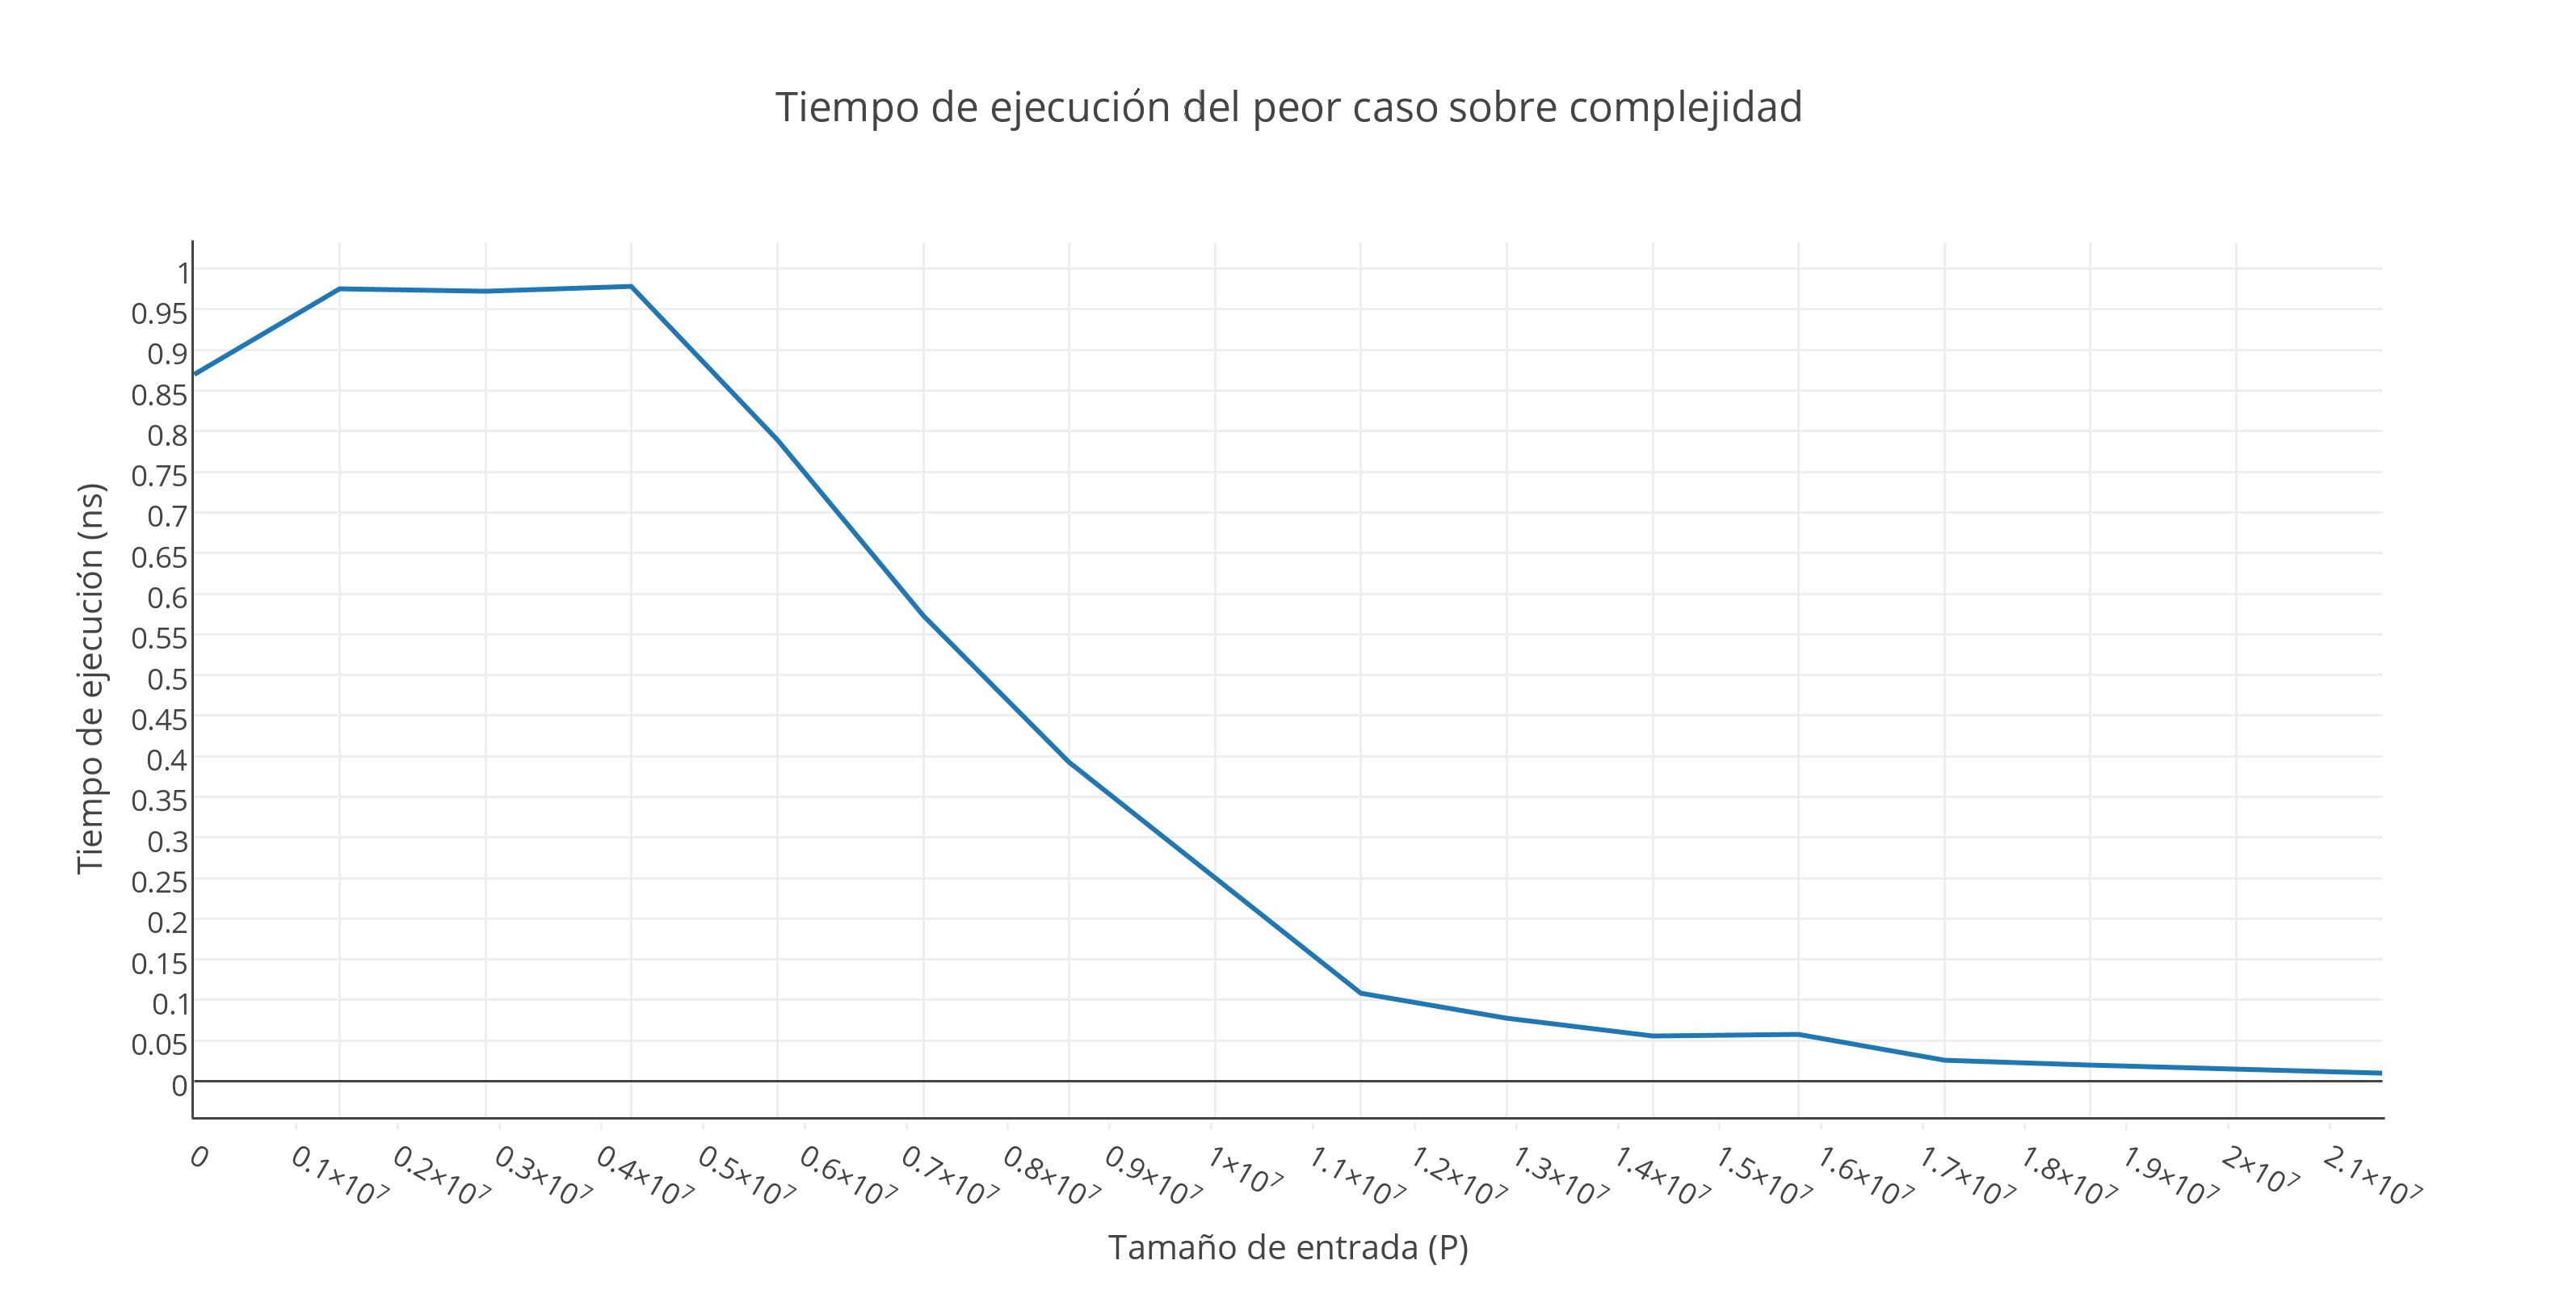
\includegraphics[scale=0.65]{./EJ2/peorcaso2.png}
 {$Gr$\'a$fico$ \ 2.7 - $Peor Caso / Complejidad$ $O(\sqrt{P})$}
  \end{center}
  \vspace*{0.3cm}

\vspace*{0.3cm} \vspace*{0.3cm}
  \begin{center}
 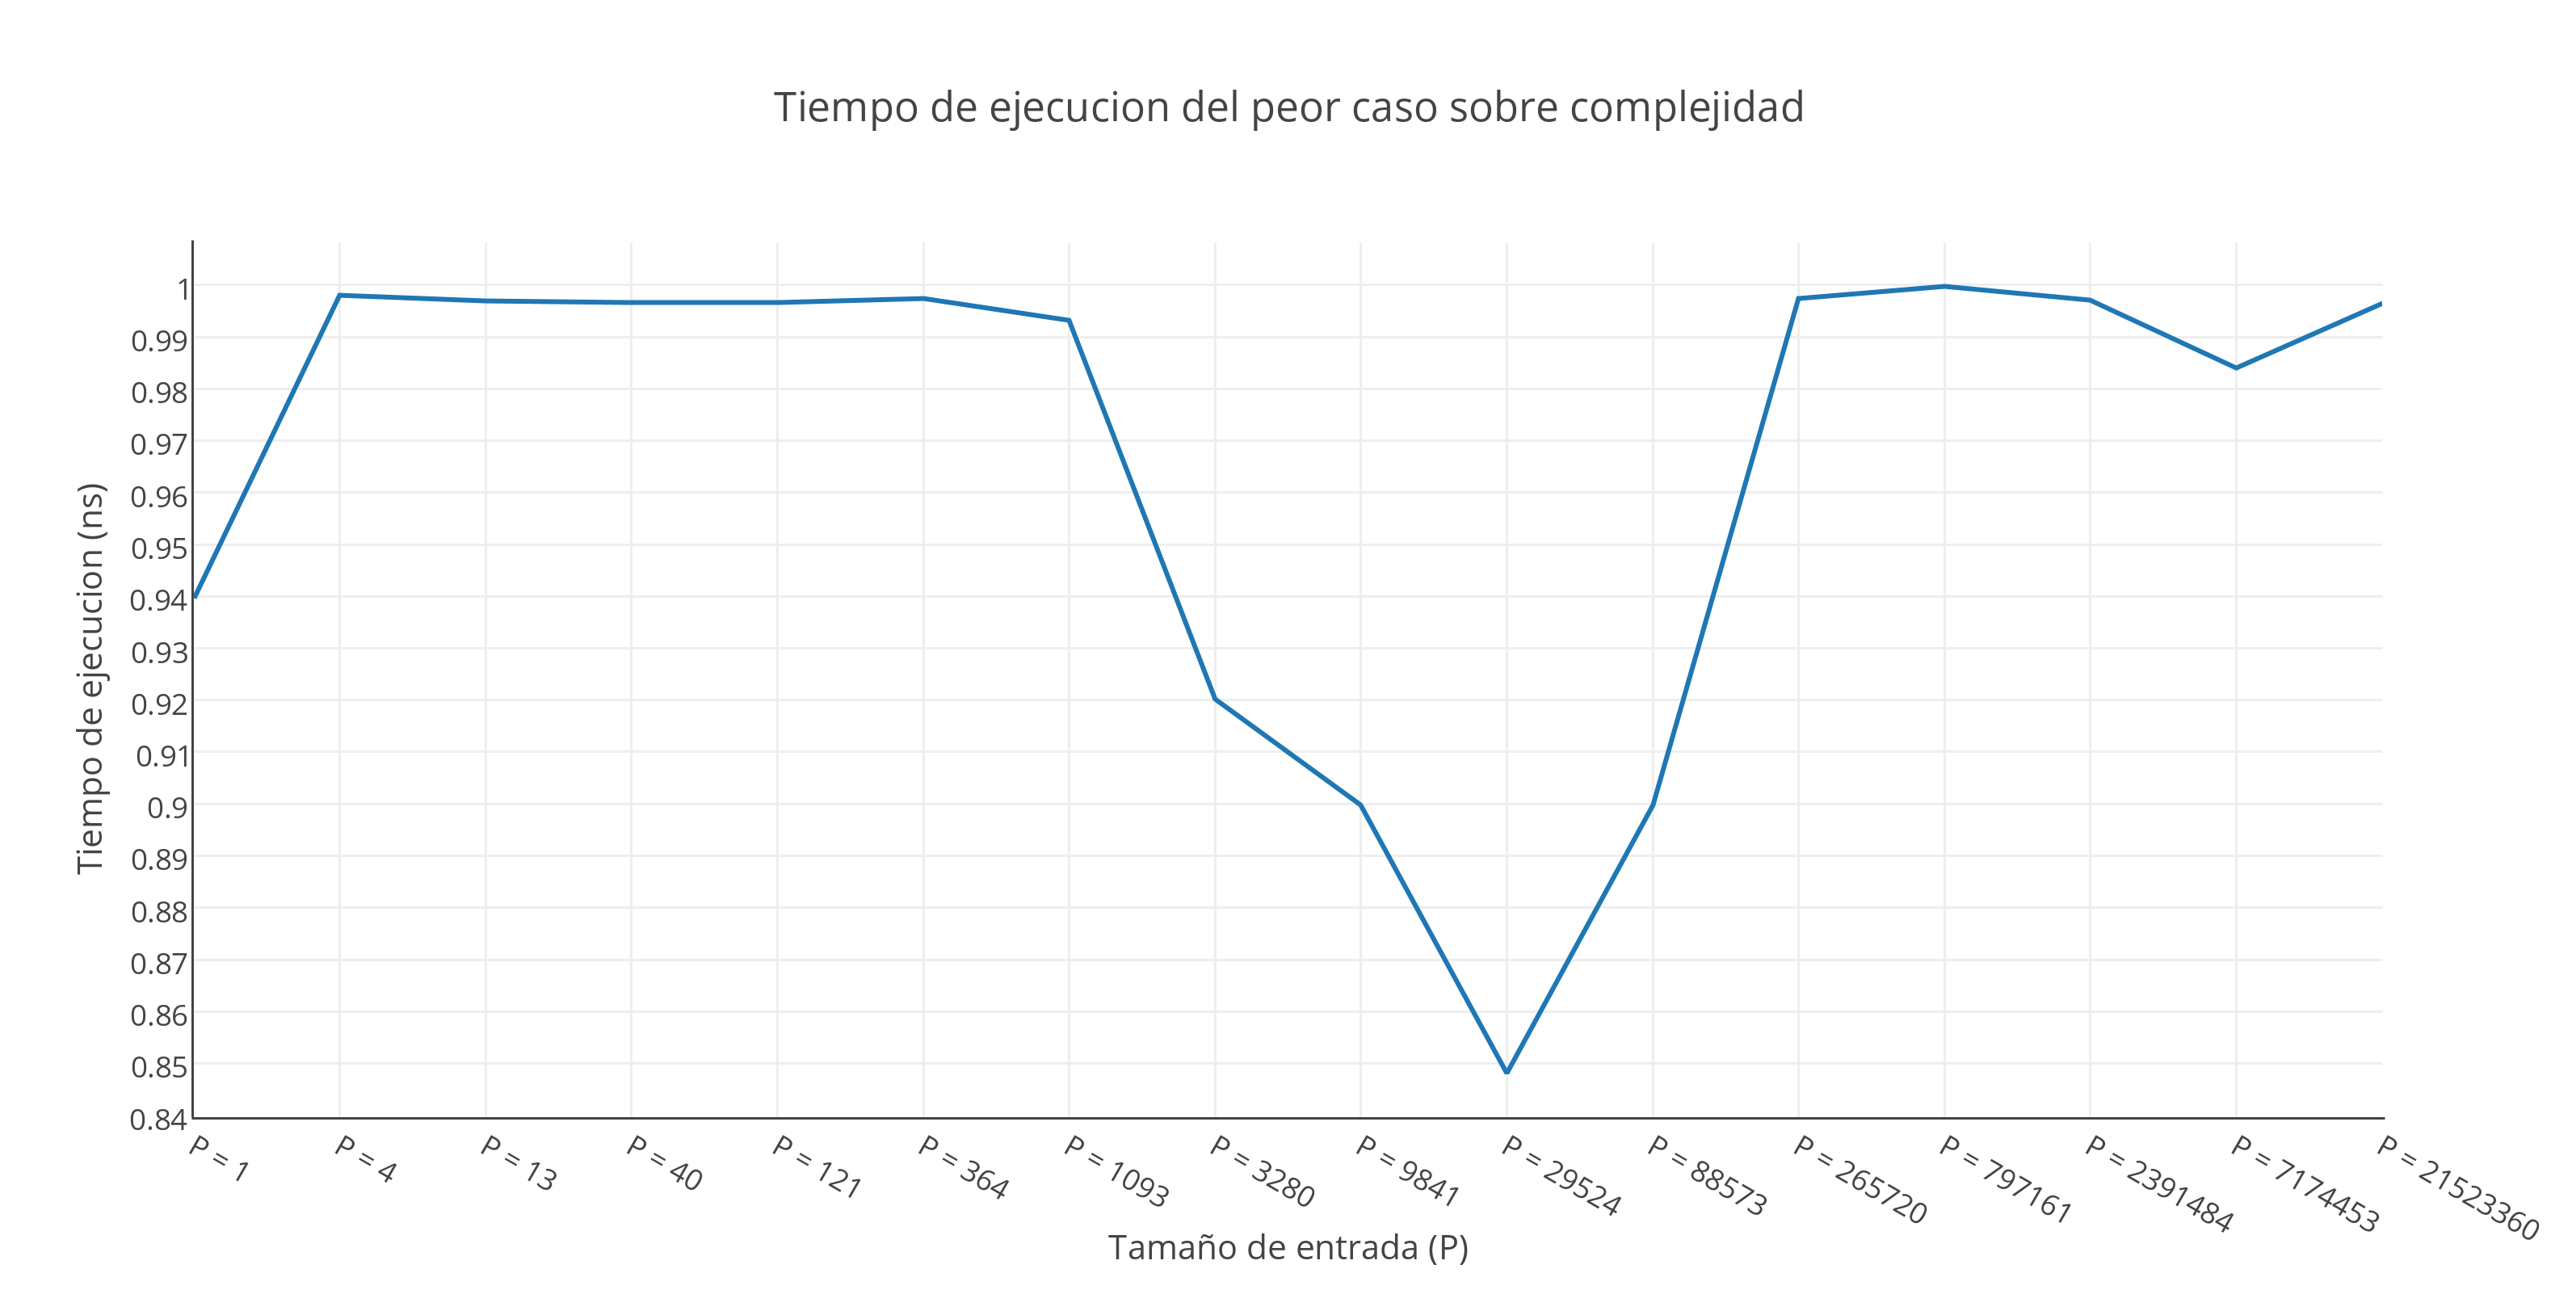
\includegraphics[scale=0.65]{./EJ2/peorcaso3.png}
 {$Gr$\'a$fico$ \ 2.8 - $Peor Caso / Complejidad$ $O(log(P))$}
  \end{center}
  \vspace*{0.3cm}

Para realizar esta experimentaci\'on nos parecio acorde, realizar un promedio con el mismo input de aproximadamente 20 corridas
tanto para la complejidad como para nuestro algoritmo y una vez calculado dicho promedio de ambas cosas realizamos la divisi\'on para
obtener resultados m\'as relevantes.\\ 

Como se puede observar en el gr\'afico 2.6 y  2.7, la funci\'on resultante de nuestro algoritmo es considerablemente mejor que la de la cota teorica $O(\sqrt{P})$ y presenta un tiempo similar al de la funci\'on resultante de la cota $O(log(P))$. Al igual que en el mejor caso, se gr\'aficaron las primeras instancias para que el gr\'afico pueda ser m\'as legible.
Luego, en el gr\'afico 2.8 a pesar de tardar varios nanosegundos m\'as que en el mejor caso, al dividir por la complejidad teorica
la función resultante tambi\'en tiende a 0 quedando comparativamente por encima del mejor caso.\\

Por \'ultimo, mostraremos un gr\'afico comparativo entre el mejor y peor caso contra la complejidad que se solicito y la demostrada la cual es considerablemente inferior:\\

\vspace*{0.3cm} \vspace*{0.3cm}
  \begin{center}
 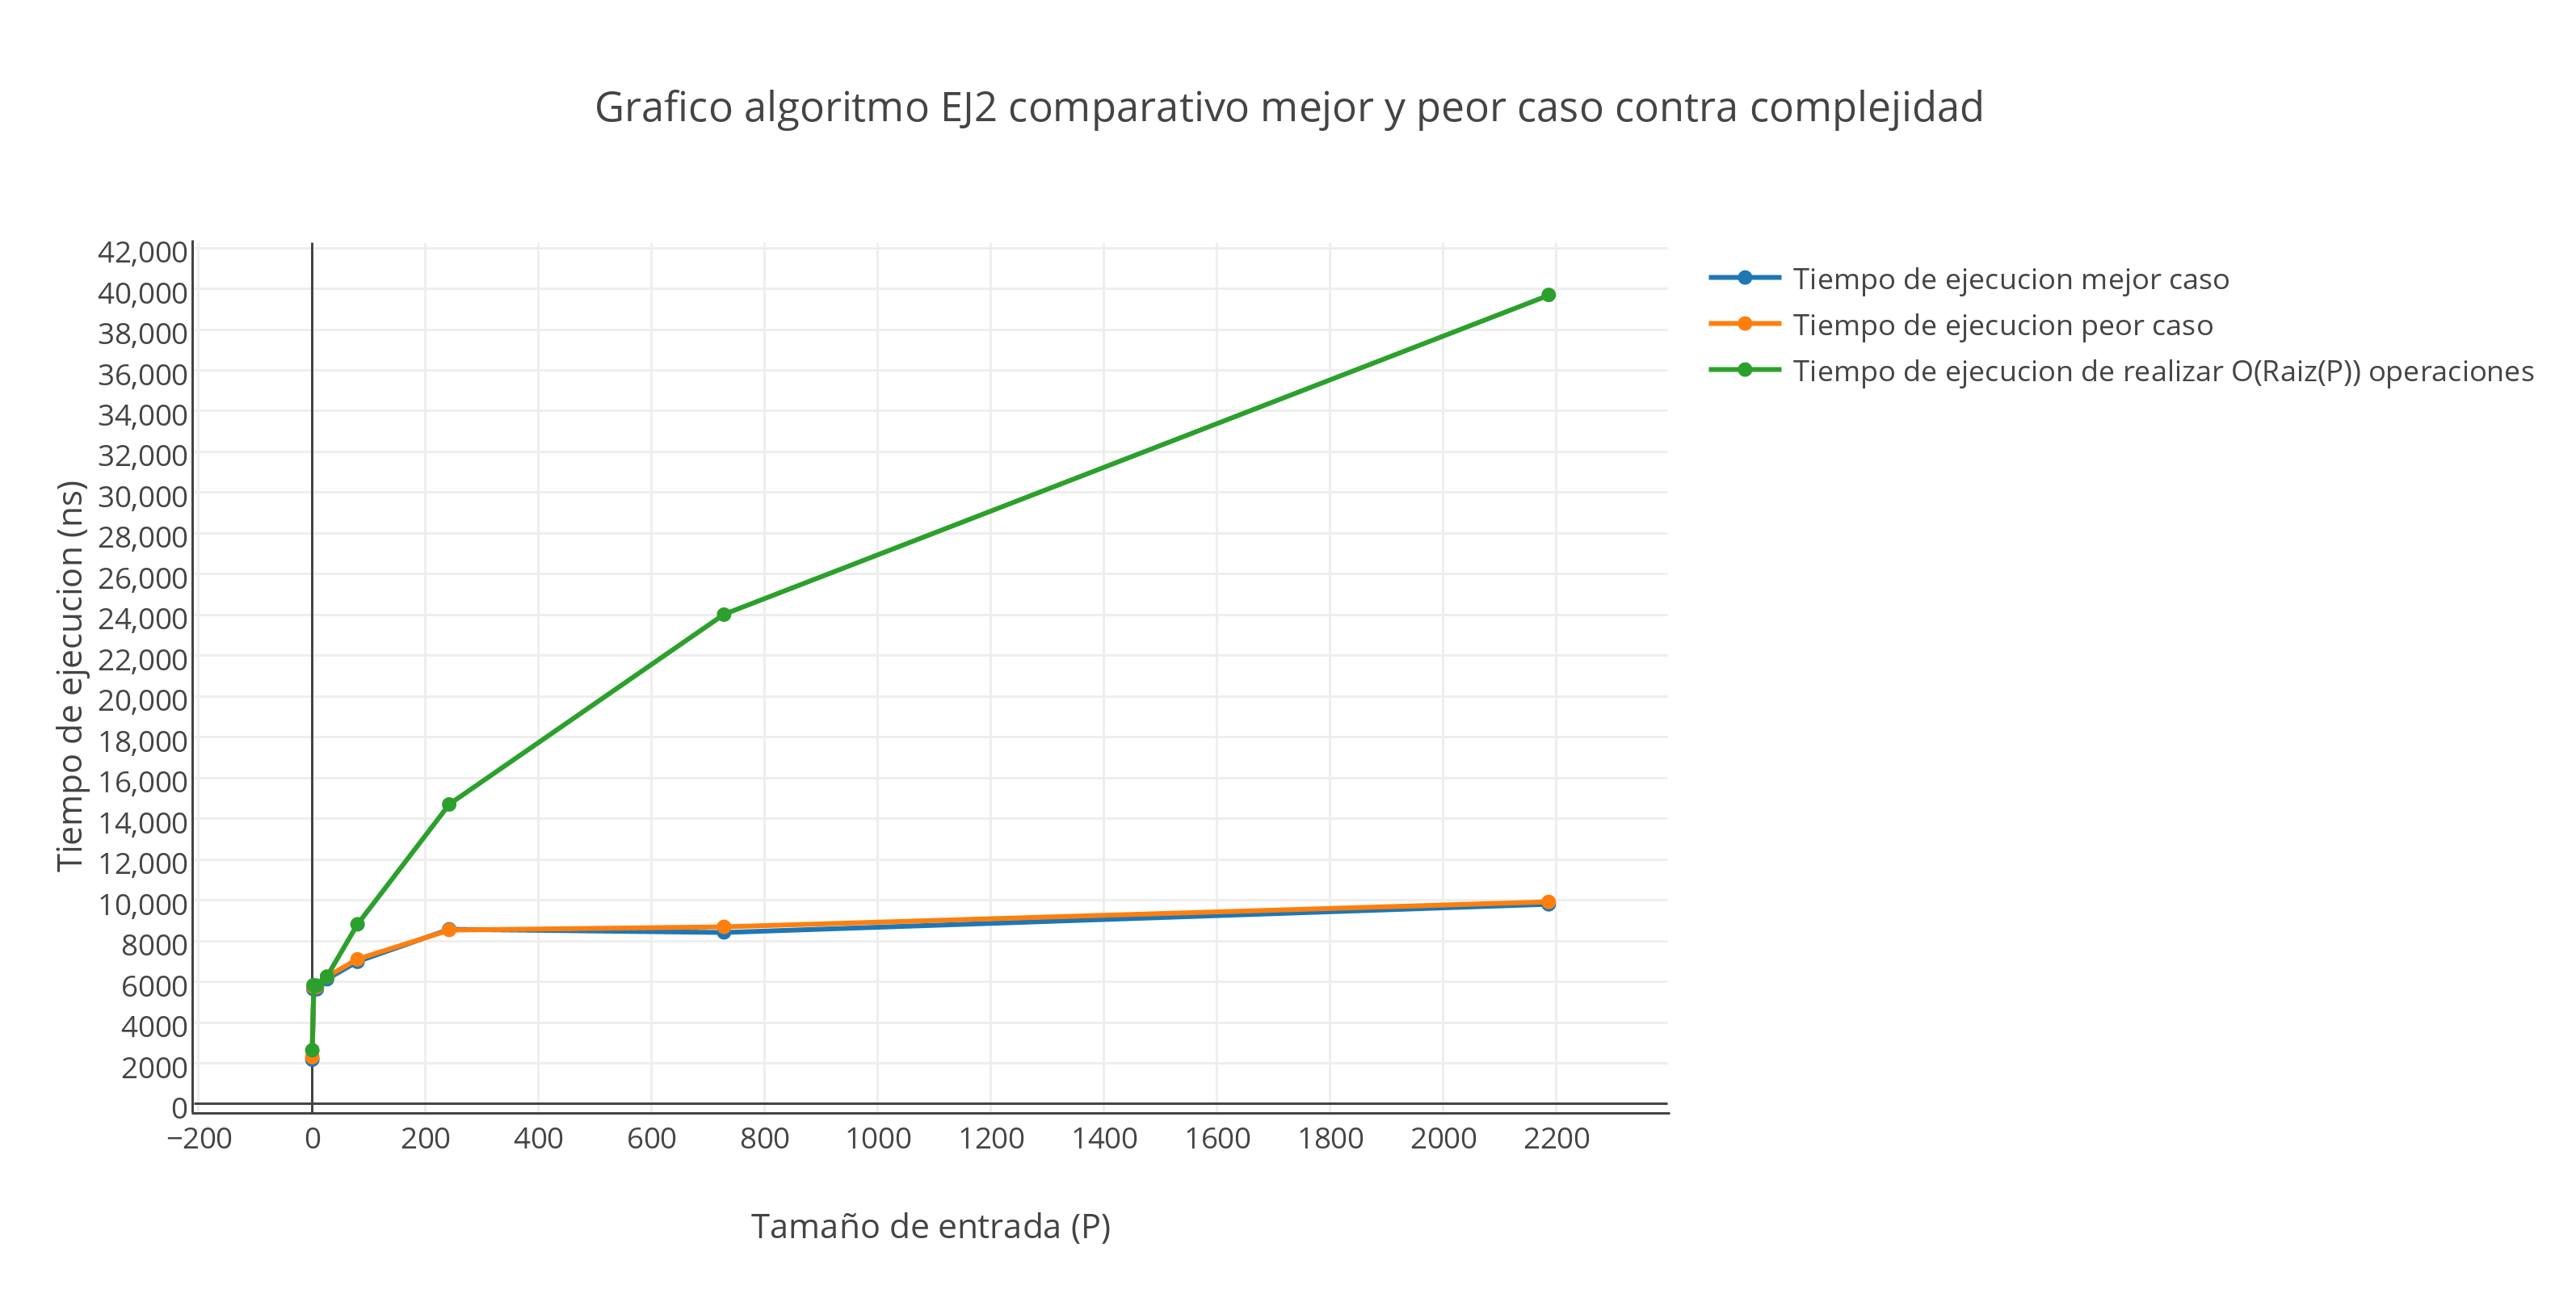
\includegraphics[scale=0.65]{./EJ2/comparativo1.png}
 {$Gr$\'a$fico$ \ 2.8 - $Comparativo$}
  \end{center}
  \vspace*{0.3cm}
  
  \vspace*{0.3cm} \vspace*{0.3cm}
  \begin{center}
 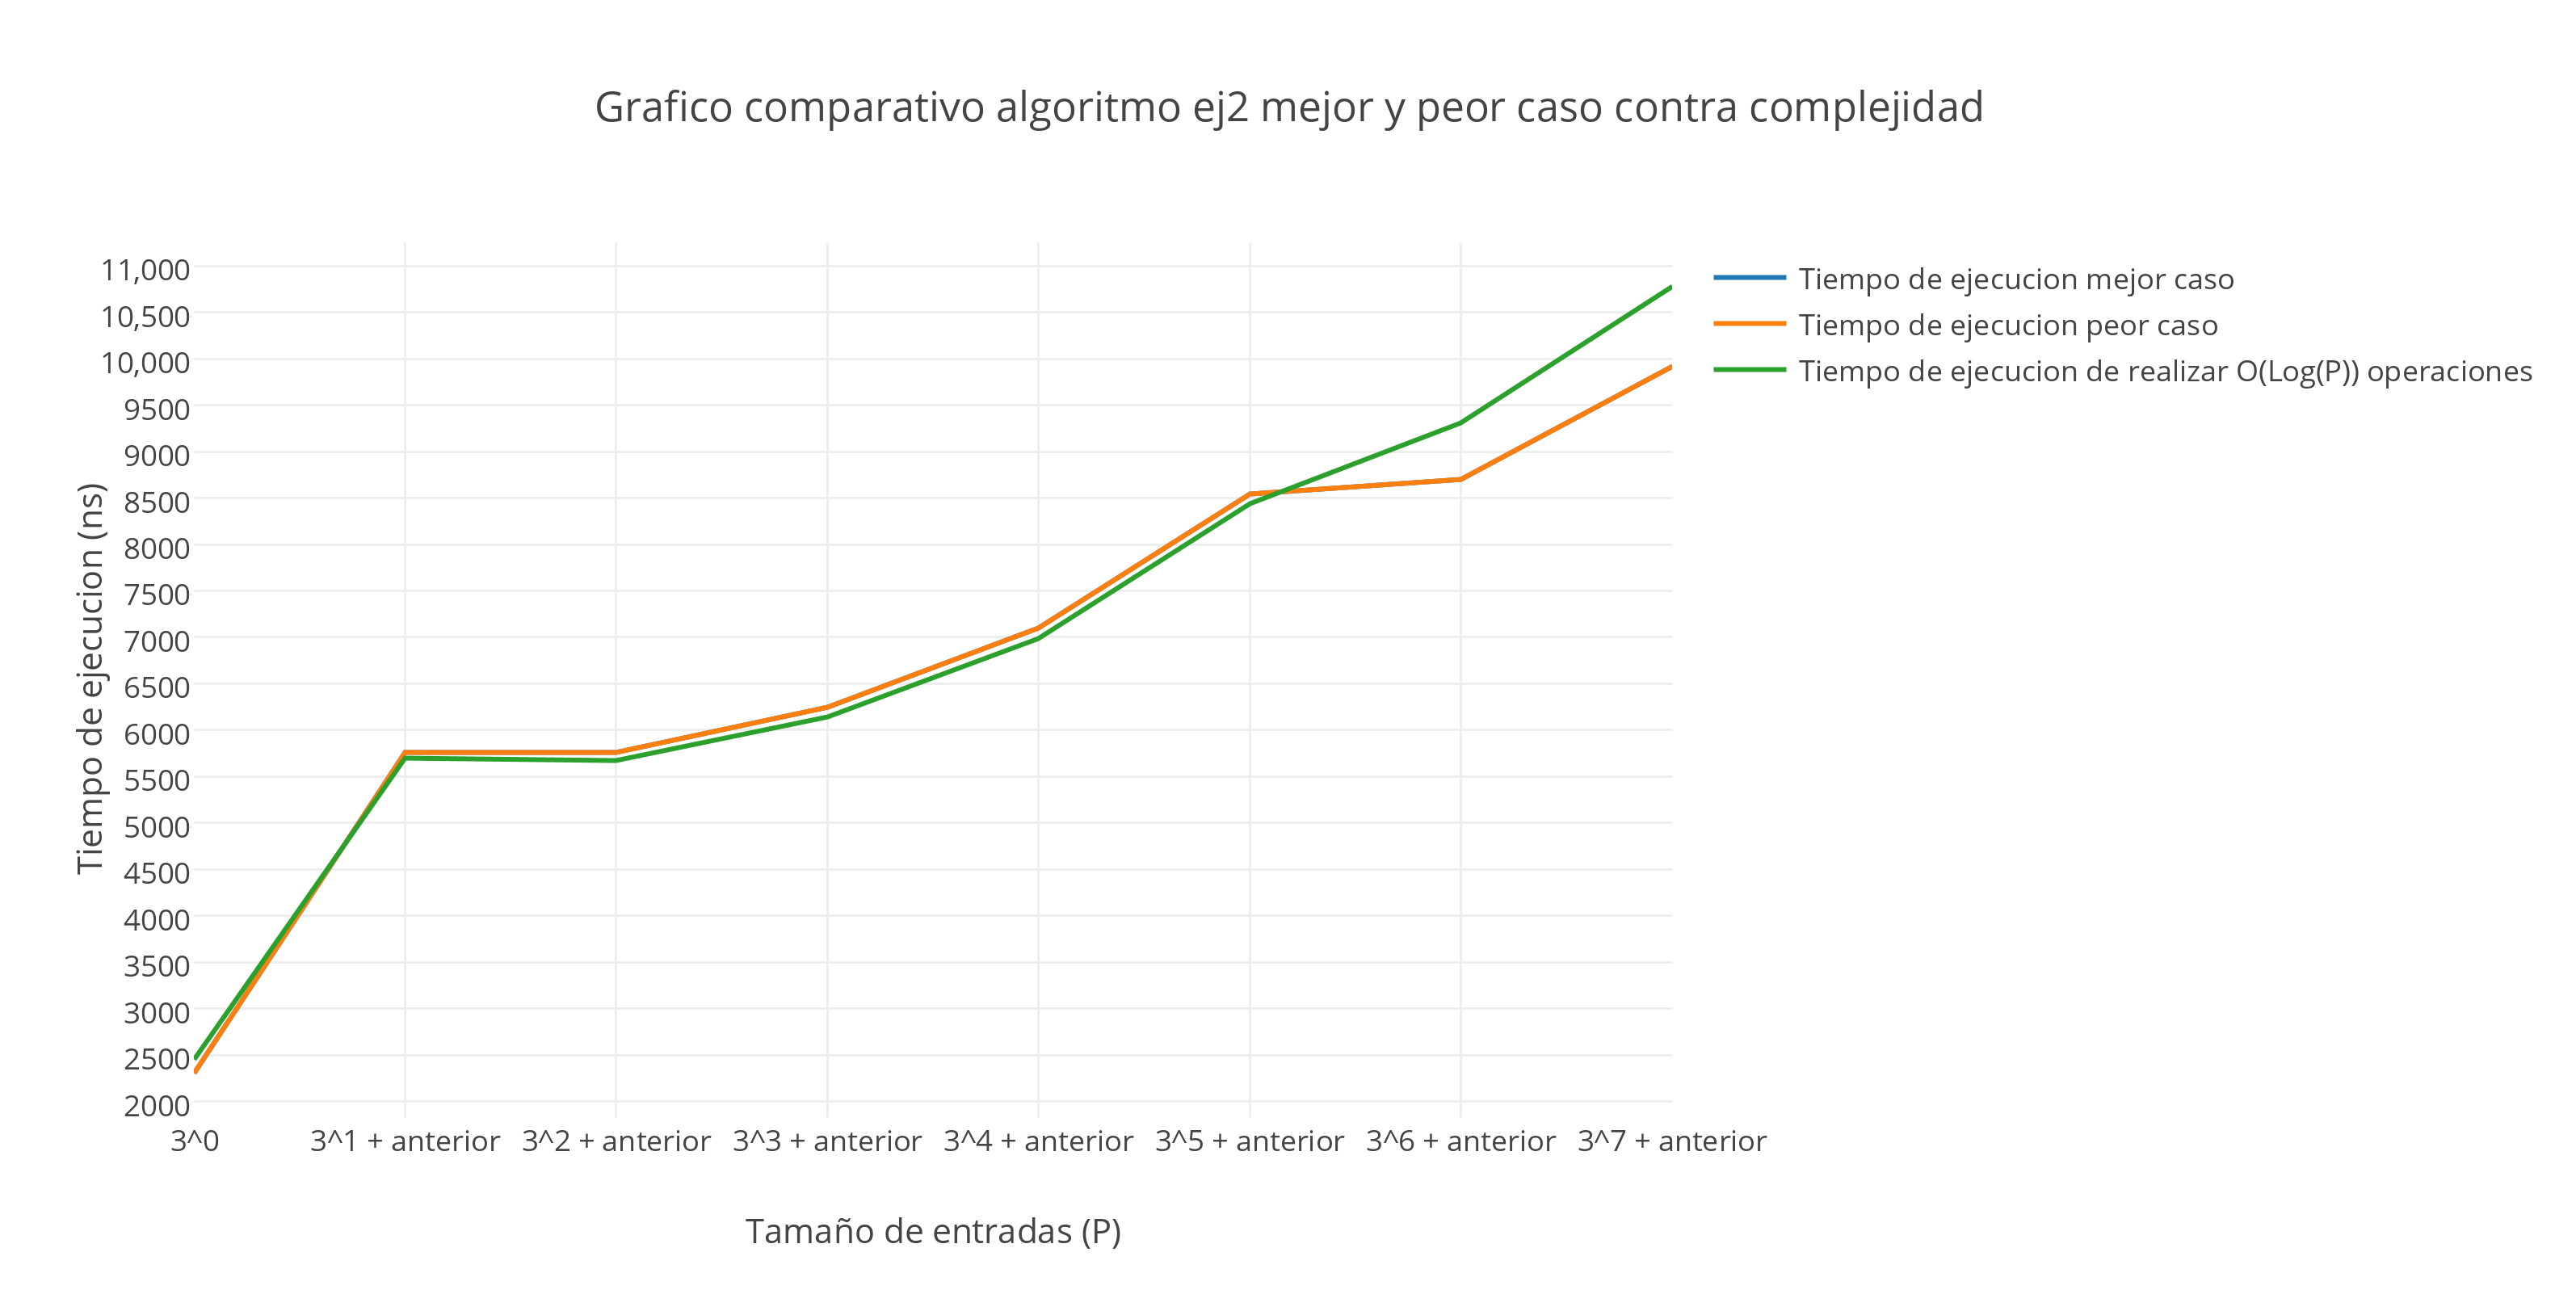
\includegraphics[scale=0.65]{./EJ2/comparativo2.png}
 {$Gr$\'a$fico$ \ 2.9 - $Comparativo$}
  \end{center}
  \vspace*{0.3cm}

Luego de dichos experimentos y casos probados, se puede concluir que a pesar de utilizar todas las pesas como en el peor caso nos mantenemos dentro de la complejidad propuesta como hab\'iamos mostrado en nuestro desarrollo de la complejidad.\\
